\chapter{The role of vertical structure in QBO teleconnections}
\label{cha:deepQBO}

\section{Introduction}
\label{sec:deepQBO-introduction}

Findings from chapter 3 indicated an association between a vertically integrated QBO index and the vortex. While a large body of work has aimed to understand teleconnections between the equatorial winds and the vortex (see section \ref{sec:external_influence_HT}), aspects of the connection between the QBO and other parts of the stratosphere as well as the troposphere and surface, evade definitive explanation.

The QBO is typically defined by the equatorial ZMZW at a single level in the mid-stratosphere and the 50 hPa level is usually used for observational studies into teleconnections between the QBO and NH variability \citep{baldwinQuasiBiennial2001}. However, some studies have also noted the importance of characterising the vertical structure of the QBO \citep{Fraedrih1993, Wallace1993,  Baldwin98,  Dunkerton2017, graySurface2018, andrewsObserved2019}. In an observational-based study \cite{graySurface2018} find an enhanced association between the QBO and polar vortex as well as MSLP anomalies over the NH when a metric incorporating the vertical coherence of equatorial winds via empirical orthogonal functions is utilised (such an EOF method is first presented in \citep{verena2016a}). The same work proposes three distinct physical pathways by which the QBO exerts influence over tropospheric and surface variations: First, via modulation of NH winter vortex strength (the HT effect, see section \ref{sec:external_influence_HT}) and the subsequet downward propagation of NAM anomalies from the vortex to the surface (see section \ref{sec:Downward_influence}. Second, through influence over tropical upwelling brought about by the induced meridional circulation associated with different QBO phases as seen in the observational study of \cite{liessRelationship2012}. Finally, via alterations in horizontal temperature gradients in the tropospheric subtropical jet region also caused by the induced meridional circulation, an effect suggested in modelling \citep{garfinkelInfluence2011} and observational studies. The same work shows that the nature of responses in the vortex and surface to the QBO vary significantly within the NH winter season with midwinter responses (in January) sensitive to QBO winds near 50hPa in contrast to early and later winter (February and March) responses which are most sensitive to the QBO defined at 20hPa and 70hPa. In a subsequent model-based study \cite{andrewsObserved2019d} introduce a similar but simpler methodology by defining the QBO as the average ZMZW between two vertical levels, which preferentially selects time intervals that display a vertically coherent QBO phase between the specified levels. The same study reports enhanced responses to the QBO from the NAO and Arctic Oscillation (AO) when such vertically integrated metrics are used to define QBO phase compared to a single level definition. However, this work does not analyse the pathways responsible for the enhanced surface response (i.e. whether the vortex response to a deep QBO is also enhanced) and the mechanisms involved in the association is still not well understood. 

In addition to the QBO, variations in ZMZW in the upper stratosphere and lower mesosphere, the SAO (see section \ref{sec:equatorial_strat}), also shows associations with the vortex. The influence of the SAO on vortex variability and SSWs was first hypothesised in the observational study of \cite{grayData2001} which used rocketsonde data to establish a link between the vertical extent of the westerly SAO phase and vortex strength. However these results statistically significant and the work stressed the need for more study with comprehensive observations as well as model simulations. Subsequent studies found similar links but with varying features. \cite{grayinfluence2003} found influence of upper stratosphere equatorial winds and SSWs over the whole season but mostly in mid winter. This was attributed to timing of the phase transition from westerly to easterly SAO. \cite{grayData2001} and \cite{hamiltonEffects1998} suggest that equatorial winds at all stratospheric levels (including the QBO and SAO regions) influence the vortex and a combination of QBO and SAO conditions is required to obtain a significant signal in vortex variability.

While many studies highlight statistical associations between QBO metrics as well as the SAO with other parts of the climate system, they are less effective at demonstrating causal relationships. Indeed, \cite{andrewsObserved2019d} note the possibility that both the occurrence of deep QBO phases and NAO and AO anomalies may be driven by an unidentified third factor which gives rise to a robust statistical link between the phenomena without any direct physical connection. Studies which utilise observation based datasets to examine the QBO-NAO/AO interaction are hampered by record length as well as the intrusion of other forcing factors associated with NH surface variations which obscure the signal from the QBO. These include Solar cycle variability \citep{GrayElevenyear2016}, volcanic eruptions \citep{stenchikovArctic2004}, in particular stratospheric injection of aerosols as well as surface variability in other regions such as ENSO \citep{bellStratospheric2009}. Some studies aim to overcome these potential pitfalls and explicitly test the nature of teleconnections with forced model setups, where momentum forcing or nudging is applied to winds in specific regions of the atmosphere. Such works further suggest the importance of the SAO and QBO region when considering the vortex. \cite{pascoeQuasibiennial2005b} finds improved vortex representation in model runs with forced winds in the equatorial stratosphere (both QBO and SAO regions separately) and \cite{grayForecasting2020} shows that nudging model winds in the SAO region (as well as specifying tropospheric wave forcing) towards reanalysis for a single winter, allows the model to capture an SSW observed in that winter with high degrees of accuracy in its timing and magnitude.   

Despite the significant body of work presented above into the QBO and its relation to other parts of the climate system, the role of vertical structure in teleconnections is not fully understood. In this chapter, we utilise a set of nudging experiments to explicitly test the importance of vertical coherence in the equatorial stratosphere's influence over the vortex as well as tropospheric and surface variability. Results form this analysis may aid in establishing the true nature of QBO teleconnections as well as develop understanding of a potentially powerful source of forecast predictive skill (the equatorial stratosphere).

\section{Model Configuration}

To explicitly test the effect of QBO vertical coherence on teleconnections we utilise a set of simulations of a modified version of the UKESM GCM analysed in chapters 3 and 4. As with the pi-control simulation examined so far, the model component for the atmosphere is GA7.1, GHG concentrations are set to 1850 levels (see section \ref{sec:model_config}) and volcanic eruptions are absent (however a constant background volcanic aerosol level is imposed). The primary difference between the pi-control and the configuration utilised here is the experiments run with no coupled Ocean component. Instead, SSTs are prescribed using a seasonally invariant climatological field obtained from an interval of the the pi-control (year numbers 96-126) \cite{oconnorAssessment2021b}. Sea Ice extents are also prescribed to climatological values using the same interval of the pi-control. All simulations are initialised using conditions from the start of the 30 year interval of the pi-control used to calculate SST and SI climatologies (year number 96). We choose to impose SST and sea ice conditions in our experiments as this removes contributions to atmospheric circulation from interannual to decadal surface modes of variability such as ENSO and the AL as well as the impact of Volcanic eruptions on stratospheric Aerosols. This in turn isolates the effect of the QBO further as any differences in QBO-vortex and QBO-surface interactions across the simulations are not due to coupling with SSTs and other surface boundary conditions. We utilise three simulations using the above configuration:

\begin{itemize}
    \item First, an unforced control simulation referred to as the \textbf{pre-industrial clim control} (pi-clim cntrl). This simulation is produced as part of CMIP6 and is run for 45 years. It is documented in full in \cite{oconnorAssessment2021b}. 
    
    \item Second, a forced run which fixes the state of the equatorial winds to a vertically coherent idealised QBO (see next section for details of idealised winds). This simulation is referred to as the \textbf{deep QBO experiment} (or simply the deep experiment) and is run for 50 years.
    
    \item A forced run which fixes the state of the equatorial winds to an idealised QBO with a low degree of vertical coherence (i.e. with opposite phases in the upper and lower stratosphere, see next section). This simulation is referred to as the \textbf{shallow QBO experiment} (or simply the shallow experiment). This simulation is also run for 50 years.
    
\end{itemize}

We choose to simulate both forced runs for 50 years to ensure the simulations cover a sufficient number of the QBO cycles to carry out a robust statistical analysis on QBO teleconnections while also working within restrictions on computing time. The pi-clim cntrl was produced as part of CMIP6 as opposed to created specifically for this analysis and was run for 45 years. This discrepancy in simulation length is relatively small and should not effect the comparison between the experiments. 


%Analysis chapters 4 and 5 showed that this year does not lie in an interval in which the QBO or the vortex exhibits significant multi-decadal oscillations. As a result, the initial conditions for the simulation are less likely samples the QBO and vortex in a randomly chosen state.

\subsection{Nudging}
In order to impose the vertical structure of the QBO in the deep and shallow QBO sensitivity experiments we employ a method to constrain atmospheric conditions in a GCM simulation known as nudging. In this method, an atmospheric quantity, $Y$, is constrained via Newtonian-relaxation which pushes the model state for $Y$ towards some imposed value at each model timestep such that

\begin{equation} \label{eq:nudging}
\Delta Y = G \Delta t (Y_{imposed} - Y_{model}), 
\end{equation}

where $\Delta Y$ is the change in $Y$ applied by the nudging scheme, $Y_{imposed}$ is the state of $Y$ from the imposed field, $Y_{model}$ is the value of $Y$ the model has evolved to since the last timestep (when it was last nudged) and $G$ is the relaxation parameter. $G$ is a measure of the strength of the relaxation towards $Y_{imposed}$ at each timestep and can also be expressed as $G = \frac{1}{\tau}$ where $\tau$ is known as the relaxation timescale. When choosing the relaxation timescale, a balance is required between constraining the model sufficiently to the imposed state (i.e. a short enough $\tau$ such that the model's $Y$ avoids evolving freely) and avoiding the introduction of large gradients (a large enough $\tau$ to avoid model instability). The MetOffice Unified model, of which the model configurations presented here are a part, typically uses a relaxation timescale of 6 hours at all vertical levels. This has been shown to produce good quality nudging results in a range of studies employing such a method despite the different radiative timescales present across atmospheric levels \citep{grayForecasting2020}. In our experiments we nudge the zonal wind, $U$, towards an idealised version of the QBO wind fields expressed as 

\begin{equation} \label{eq:imposed_U}
U_{qbo}(t, p) = F(p) sin(\frac{2\pi (t + s(p))}{period}),
\end{equation}

Where $s(p)$ is a parameter which varies with pressure level and sets the rate of phase shift with descending height. For simplicity, we choose $s(p)$ such that a linear descent rate with increasing pressure is achieved. Namely, that $s(p) = -k p$, where $k$ is a constant. We then select different values for the parameter $k$ to achieve a deep QBO and shallow QBO: For the deep experiment, $k = xx$ achieves a higher degree of vertical coherence while for the shallow experiment, $k = xxx$ which leads to a larger phase shift with descending pressure level (and therefore less vertical coherence). We choose the period of the QBO in both experiments to be 32 months for consistency with the QBO period exhibited in the UKESM pi-control which is extended compared to reanalysis (see section \ref{sec:strat_var_UKESM}). $F(p)$ is a momentum forcing vertical profile applied to reproduce the variation in magnitude of the QBO withn pressure level (the QBO peaks in magnitude at around the 20hPa level in ERA-Interim). Following the methodology of \cite{pascoeQuasibiennial2005b}, we use an $F(z)$ which takes the form of a Weibull function given by

\begin{equation} \label{eq:vertical_profile}
F(z) = R_D \frac{1}{\gamma \beta^\alpha}  Z_D^{\alpha-1}  e^{-Z_D/\beta},
\end{equation}

where the parameters are set to $\alpha = 3.5, \beta = 0.27, \gamma = 3.2335, R_D = 40.0 ms^{-1}, Z_{D} = (z - 15)/20$. The idealised time-height QBO profiles generated for both experiments are shown in figure \ref{fig:Idealised_QBO_samples}, they highlight the differences between idealised QBOs: The deep QBO winds exhibits the same sign of wind throughout the middle atmosphere for the majority of the series while the shallow QBO show different phases between the upper and middle stratosphere. In both experiments we apply the relaxation in equation \ref{eq:nudging} towards the corresponding QBO winds over the set of atmospheric levels approximately corresponding to the pressure level range 90-5hPa and the latitudinal range 10$^{\circ}$\,S--10$^{\circ}$\,N. The relaxation is applied at all longitudes. At the boundary between of these ranges we apply a tapered version of the relaxation with a value of that parameter $G$ that decreases linearly with increased distance from the relaxation region. This tapering is applied on the 2 atmospheric levels at the bottom and top of the vertical region and 5$^\circ$ either side of the latitudinal region. This tapering is applied to avoid introducing large vertical and latitudinal gradients in zonal wind and prevent potential model instability. 

\begin{figure}[h!]
\begin{center}
\noindent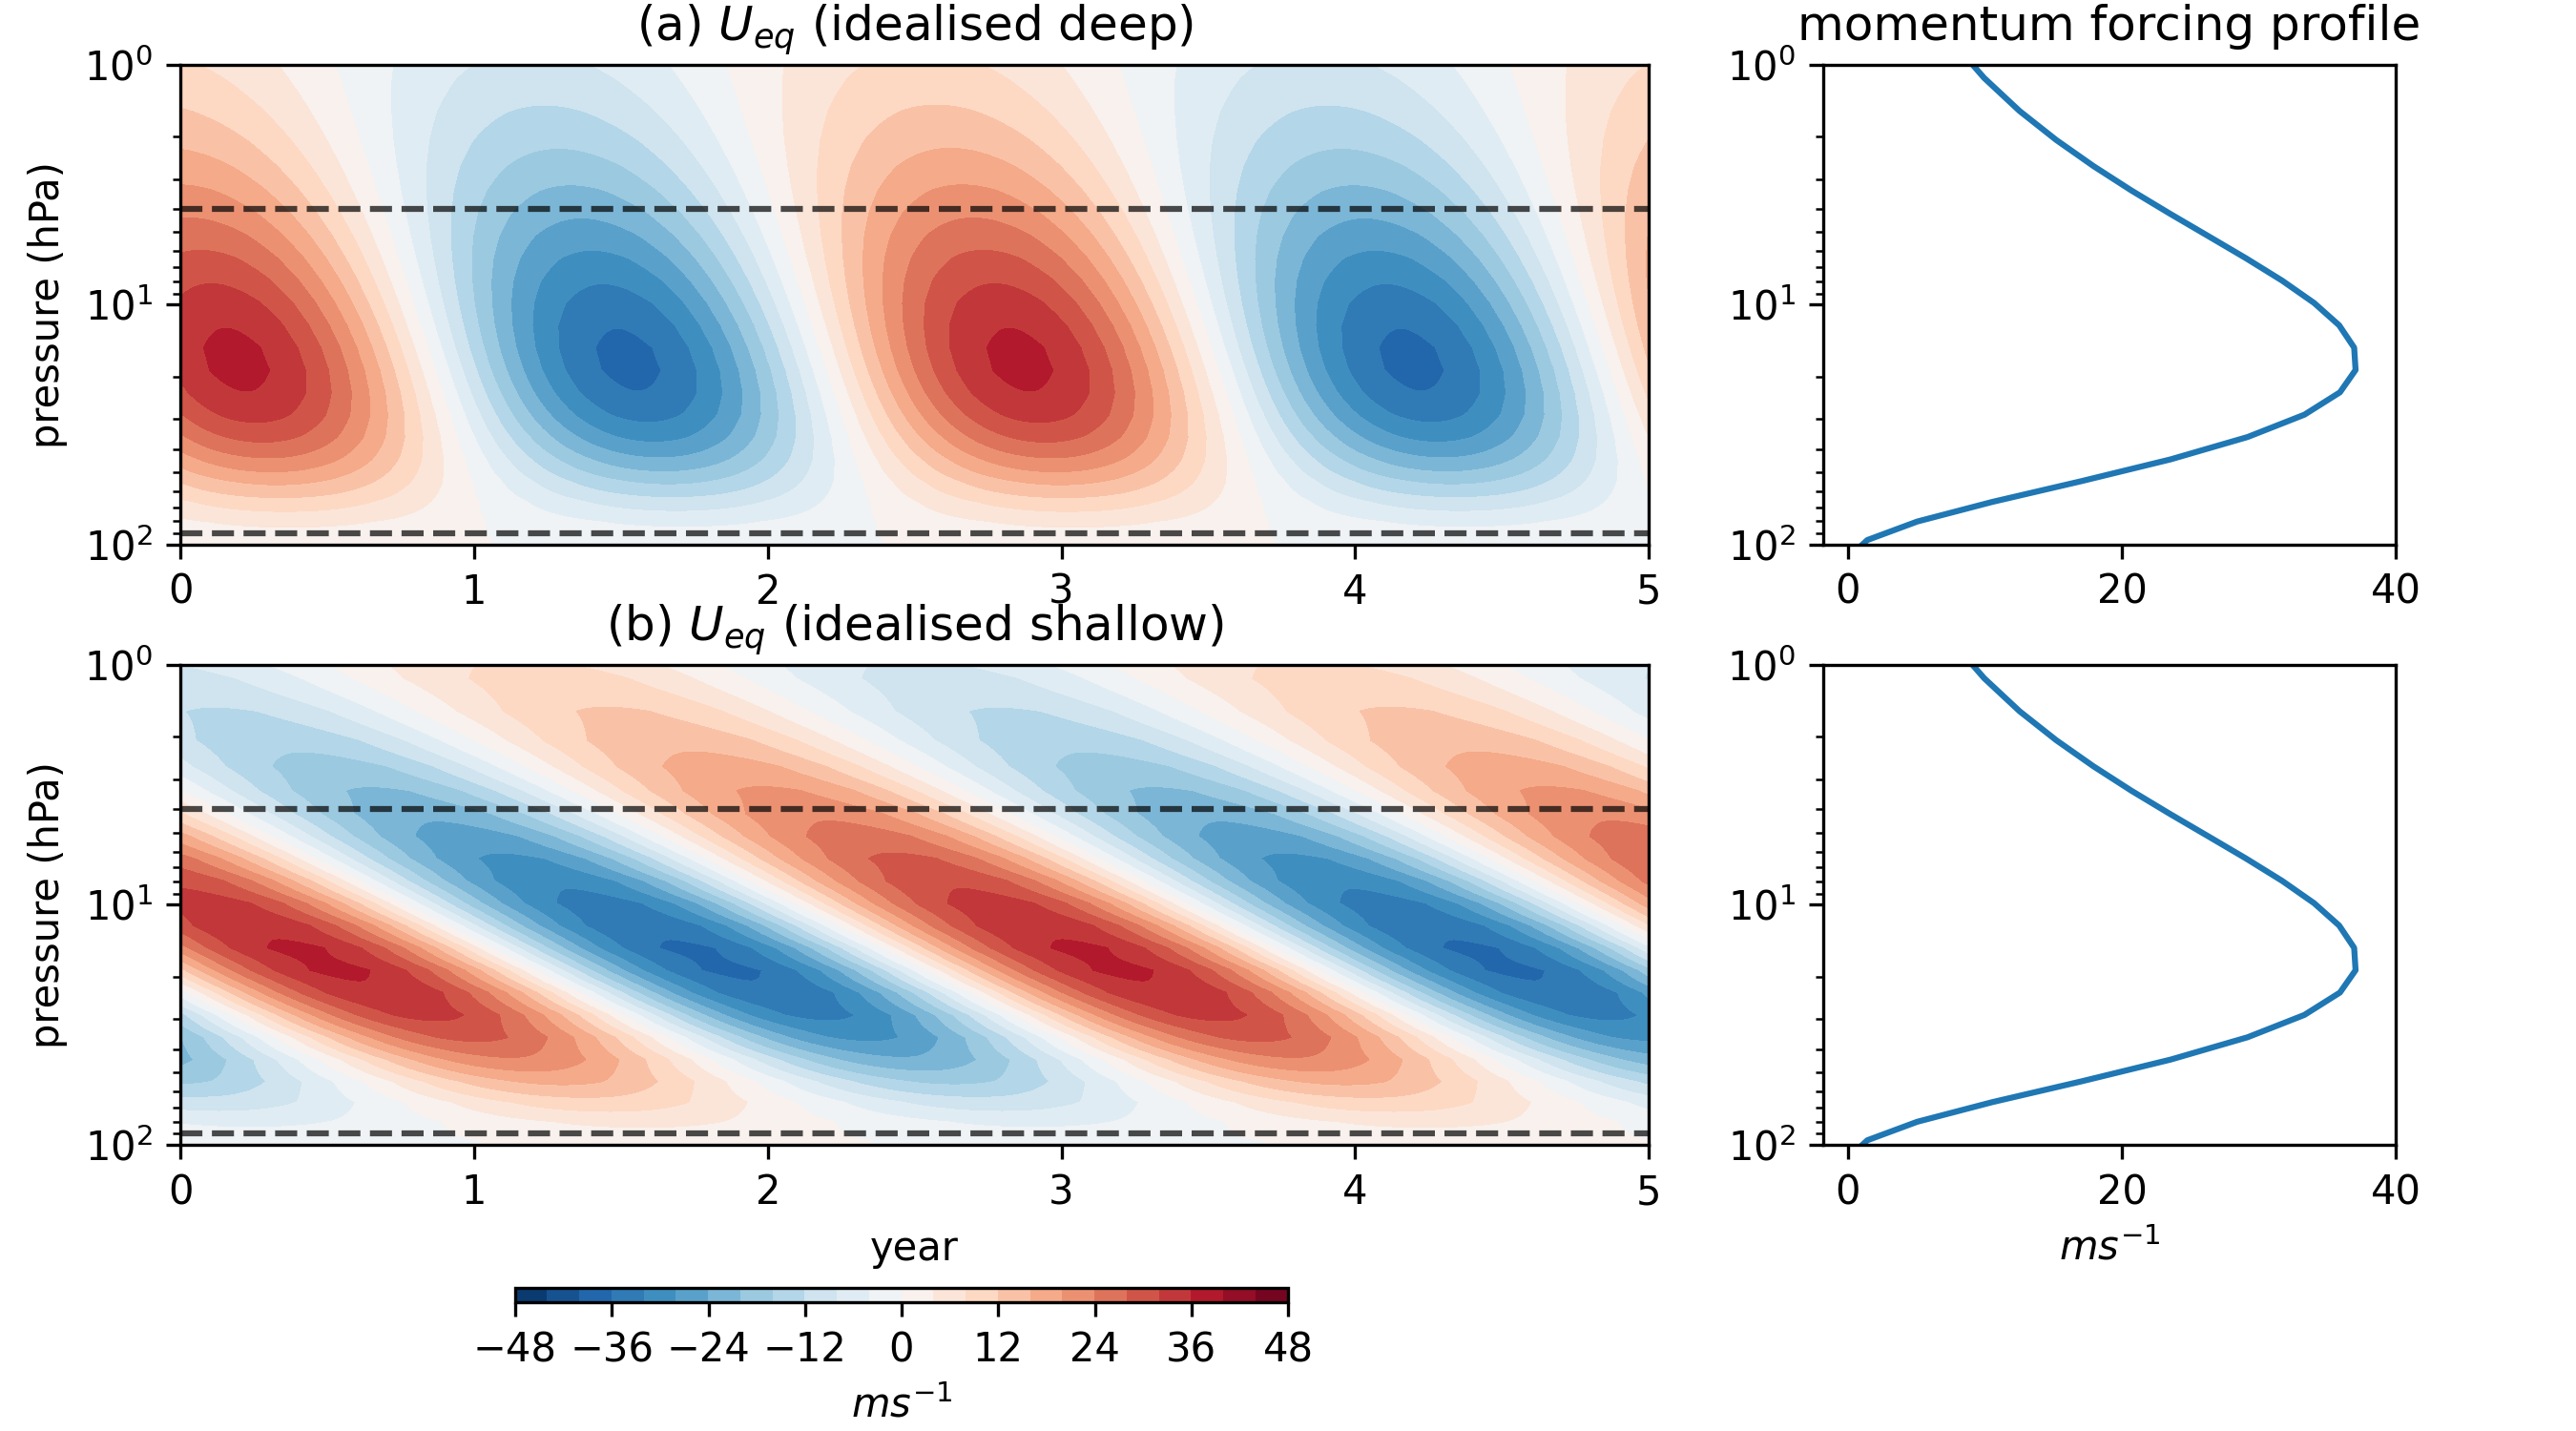
\includegraphics[width = \linewidth]{Figures/Figures-deepQBO/Idealised_QBO_features.png}
\caption[Idealised QBO winds used for nudging experiments]{Sample time-series of idealised equatorial ZMZW and associated momentum forcing profile for the deep (\textbf{a} and \text{b} respectively) and shallow (\textbf{c} and \textbf{d} respectively) QBO experiments. Horizontal dashed lines on (a) and (c) denote the xxhPa and 90hPa pressure levels between which we implement nudging towards the idealised wind in each experiment.}
\label{fig:Idealised_QBO_samples}
\end{center}
\end{figure}


\section{QBO Characteristics}
We first analyse the equatorial winds in each experiment and verify whether the implementation of nudging has resulted in the desired equatorial ZMZW profiles. Figure \ref{fig:experiment_QBOs}a and c show a 5 year sample of the the equatorial winds in each experiment that results from implementing QBO nudging between the 90hPa and 5hPa levels. These winds reflect many of the key features of the idealised winds (figure \ref{fig:Idealised_QBO_samples}a and c) - the deep experiment exhibits vertical coherence in the middle stratosphere while the shallow simulation shows opposite phases of the QBO in the upper and lower stratosphere. The period of ZMZW variations in both experiments is indicated by the Fourier power spectra shown in figures \ref{fig:experiment_QBOs}b and d. The mid-stratospheric winds (90-$\sim$ 10hPa) exhibits peak Fourier power corresponding to a period close to the value specified by the idealised winds (32 months) in both experiments. The QBOs produced by the nudging experiments also show good agreement in phase amplitude and period with that of the pi-clim cntrl (figures \ref{fig:experiment_QBOs}e and f): This confirms that the implementation of the nudging has retained the characteristics of the un-nudged run and only imposed the desired vertical structures.

\begin{figure}[h!]
\begin{center}
\noindent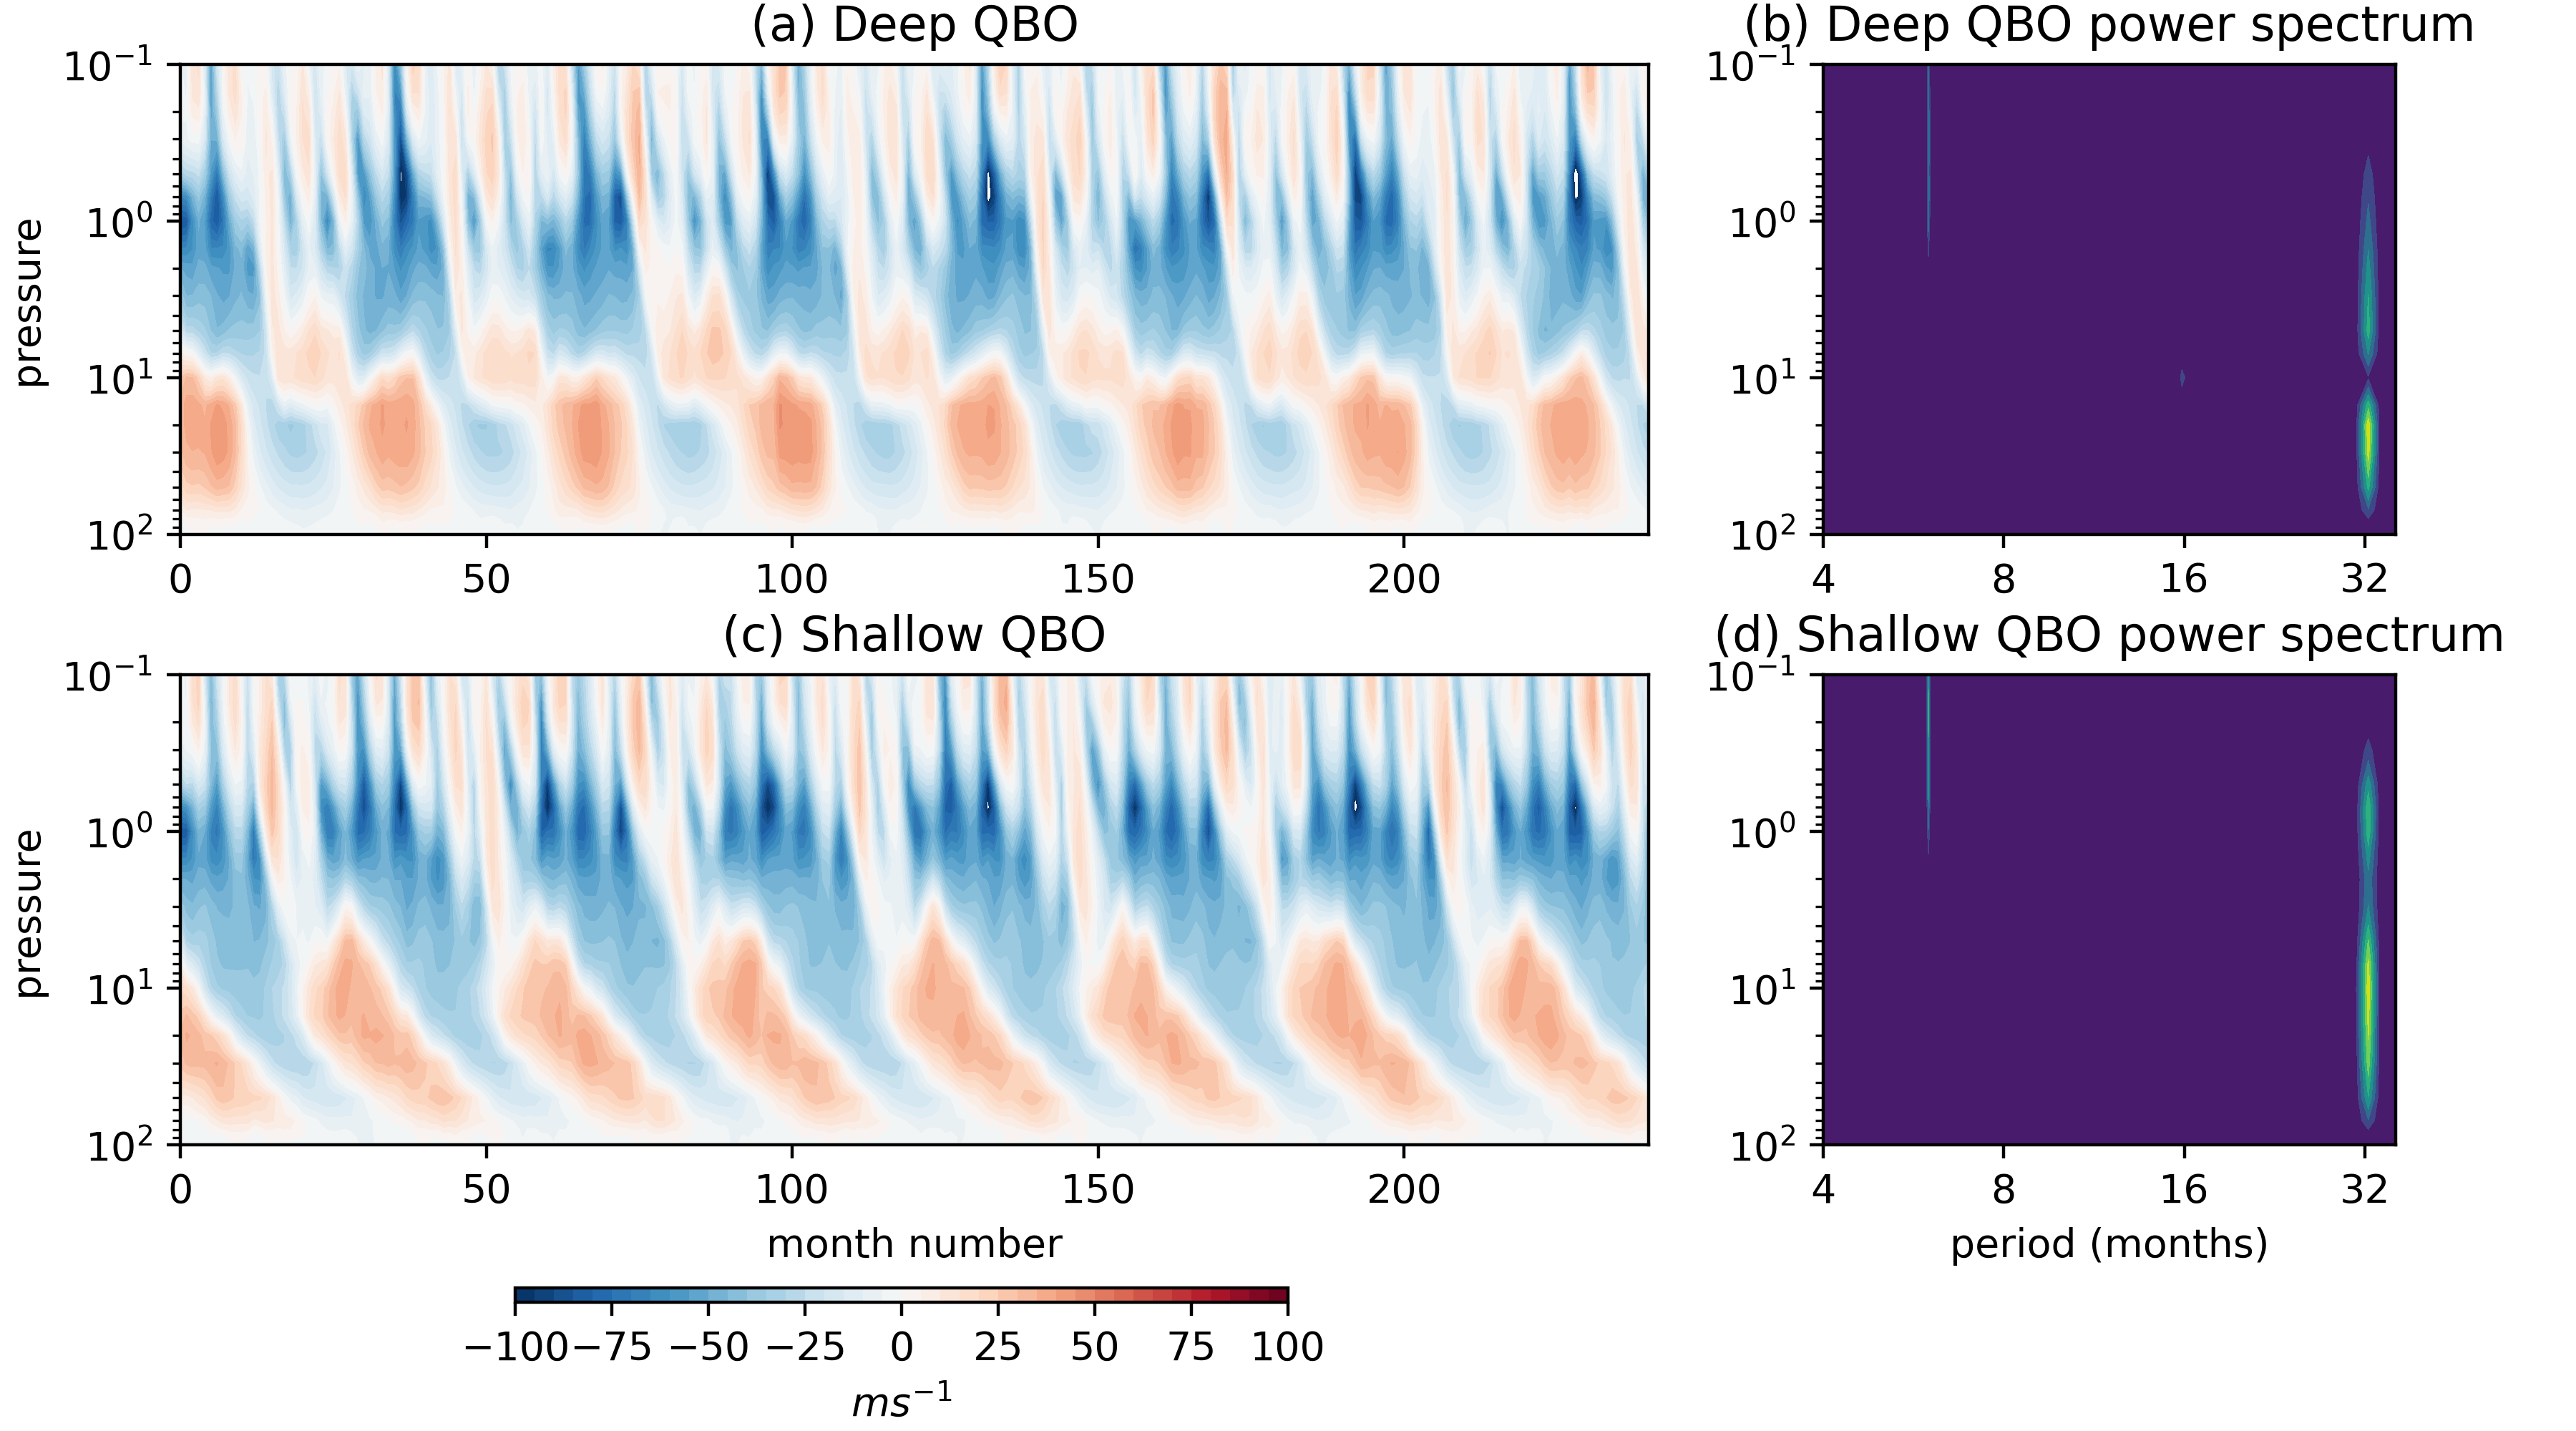
\includegraphics[width = \linewidth]{Figures/Figures-deepQBO/experiment_QBOs.png}
\caption[Equatorial ZMZW time-height profiles from QBO nudging experiments]{5 year sample of ZMZW averaged between 5$^{\circ}$\,S--5$^{\circ}$\,N latitude from the deep (\textbf{a}), shallow (\textbf{c}) QBO experiments and pi-clim control simulation (e). Thick black contours denote the 0-wind line where westerlies meet easterlies. Sub-figures b, d and f show Fourier Power spectra for equatorial winds at various levels for the deep, shallow and pi-clim control simulations respectively.}
\label{fig:experiment_QBOs}
\end{center}
\end{figure}

While the simulations' QBO reflects some of the main characteristics of the target nudging winds, there is a notable asymmetry in the amplitudes of the two QBO phases in both experiments with the westerly phase amplitude appearing larger in all QBO cycles throughout each simulation. This is an unexpected result - We defined the target nudging field using equation \ref{eq:imposed_U} which ensures each phase of the idealised QBO exhibits identical magnitude (i.e. $F(z)$ in equation \ref{eq:imposed_U} is constant in time). To examine this asymmetry further, we analyse the timeseries of simulated and idealised winds on individual pressure levels to identify potential biases (Figures \ref{fig:winds_on_levs_deep} and \ref{fig:winds_on_levs_shallow}). In the deep experiment (figure \ref{fig:winds_on_levs_deep}) the easterly phase of the QBO is in good agreement with the idealised winds on each of the pressure levels sampled. In contrast, the magnitude of the westerly phase resulting from the simulation is systematically over-represented compared to the nudging winds. This effect is apparent throughout much of the mid-stratosphere (10hPa-50hPa) and suggests the possibility of a westerly momentum forcing term in the model which acts to override the influence of the nudging scheme. This in turn may suggest that our selection of nudging timescale, $\tau$ = 6 hours, is too long in relation to other forcing terms which act on shorter timescales. The effect is less pronounced in the shallow experiment with only the QBO at 50hPa exhibiting notable over-representation in westerly amplitude. The source of additional forcing term is unclear but is likely closely associated with kelvin wave forcing as this is the primary source of the westerly QBO phase (see section \ref{sec:equatorial_strat}). While this bias does lead to marginal asymmetries in QBO phases, the desired vertical structures is obtained in both experiments which is the focus of this study and therefore we proceed with the simulations for analysis of QBO teleconnections in the next section. The possible detrimental effect of this amplitude bias is that NH winters in which we study teleconnections may preferentially occur under one QBO phase more than the other. As a result, in all future analysis of these simulations we note the number of NH winters exhibiting each QBO phase and only draw major conclusions in cases where their abundance is comparable. The result from figures \ref{fig:winds_on_levs_deep} and \ref{fig:winds_on_levs_shallow} may also indicate the suitability of a shorter nudging timescale for future nudged QBO experiments using this model setup than that recommended by the MetOffice Unified Model documentation (xxxx) but further simulations are required to confirm this.

\begin{figure}[h!]
\begin{center}
\noindent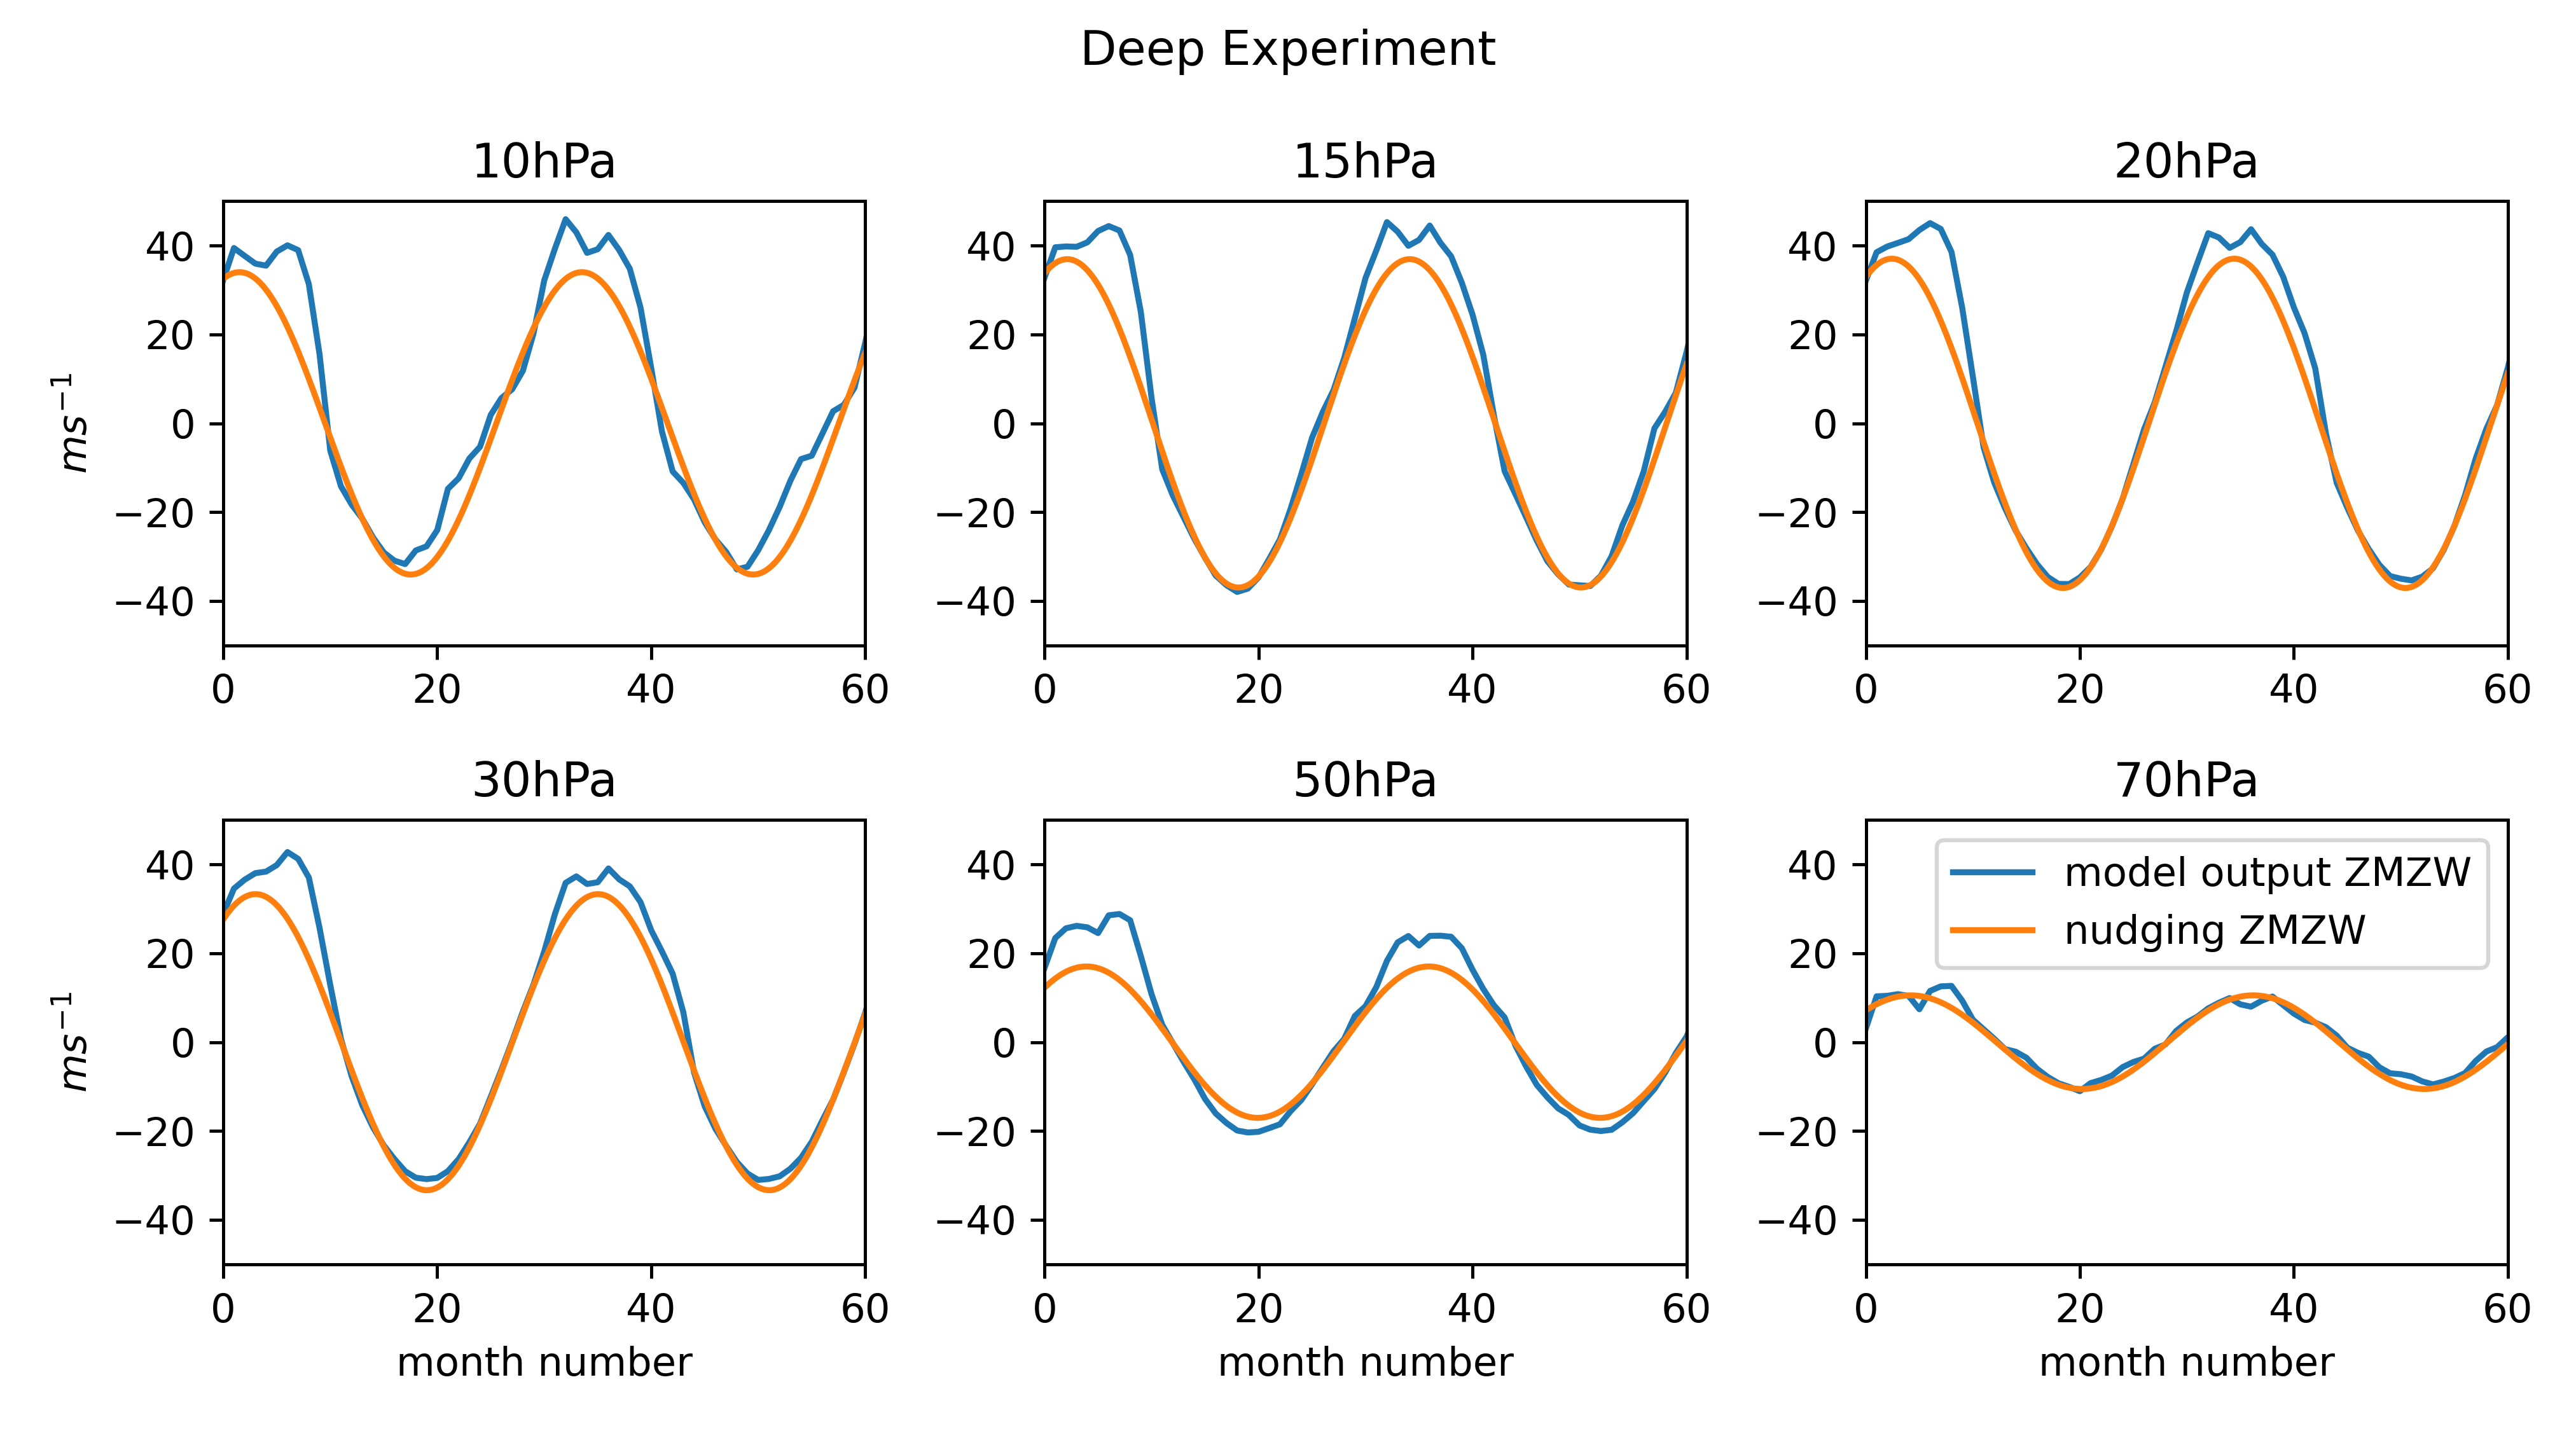
\includegraphics[width = 0.95\linewidth]{Figures/Figures-deepQBO/winds_on_lev_nudging_deep.png}
\caption[Equatorial ZMZW time-height profiles from QBO nudging experiments]{5 year sample of ZMZW on individual pressure levels averaged between 5$^{\circ}$\,S--5$^{\circ}$\,N latitude from the deep QBO experiments (blue) and the Idealised wind field used for nudging in the same experiment (orange).}
\label{fig:winds_on_levs_deep}
\end{center}
\end{figure}

\begin{figure}[h!]
\begin{center}
\noindent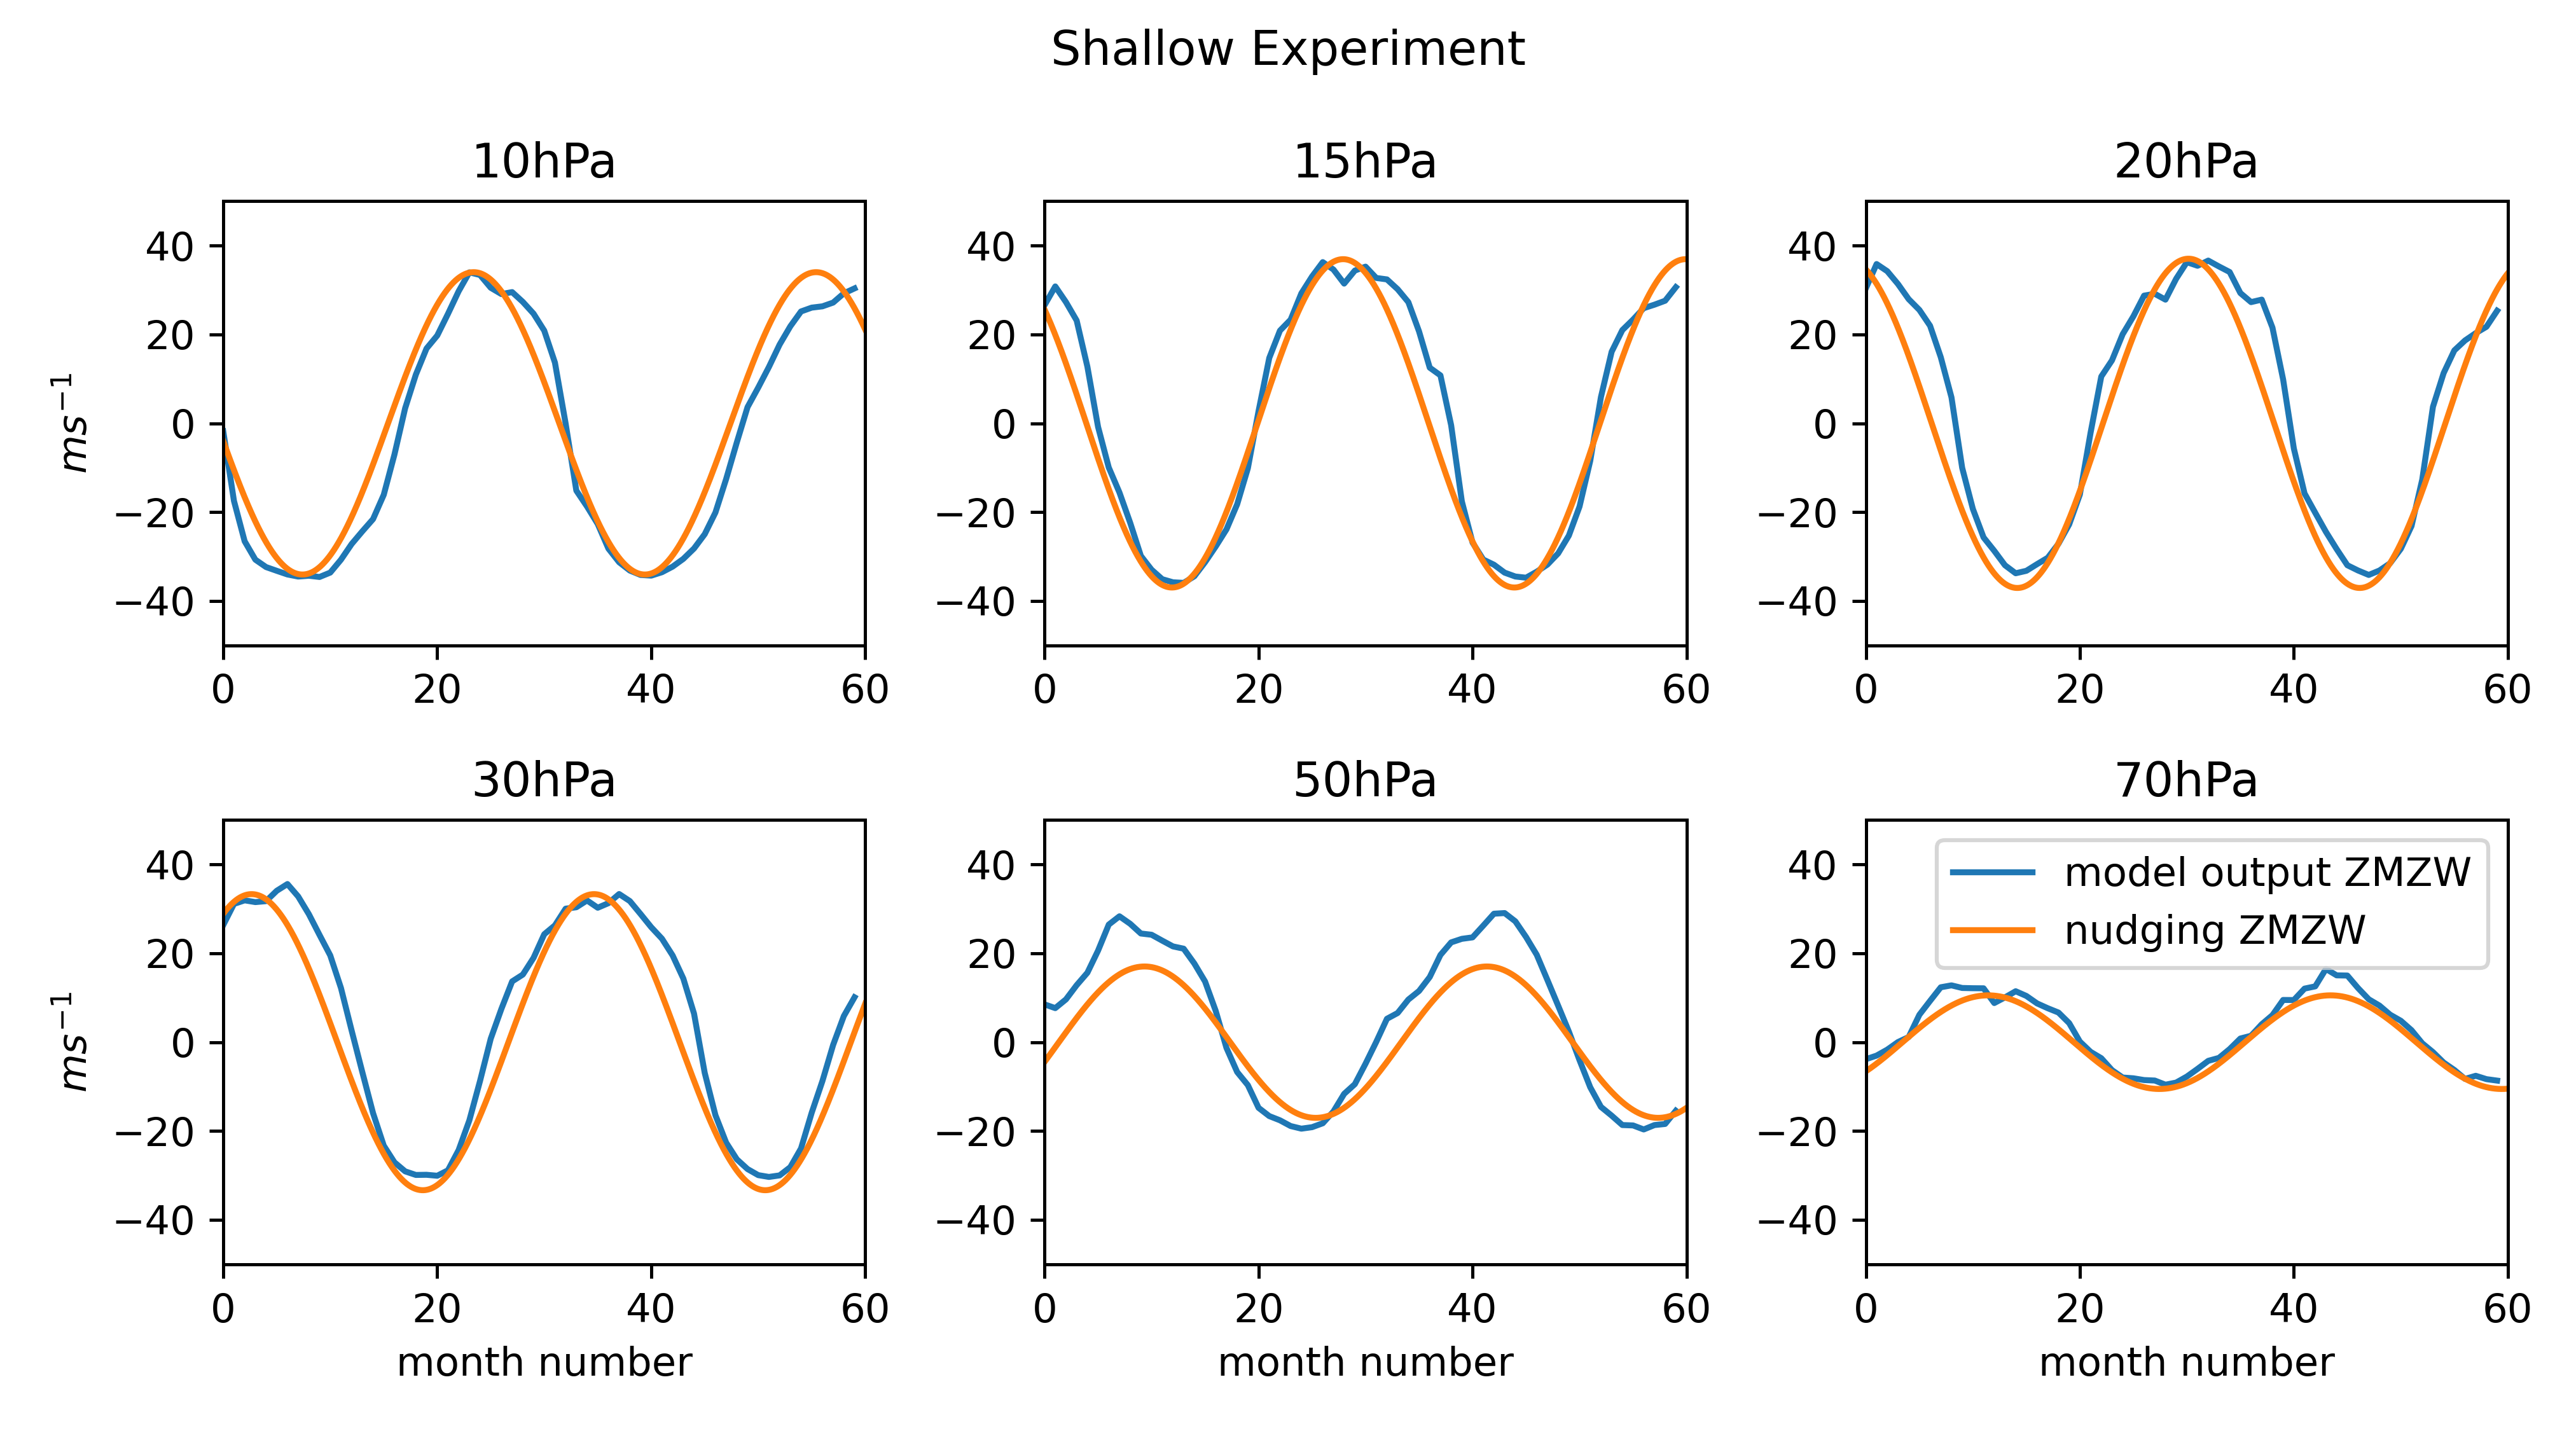
\includegraphics[width = 0.95\linewidth]{Figures/Figures-deepQBO/winds_on_lev_nudging_shallow.png}
\caption[Equatorial ZMZW time-height profiles from QBO nudging experiments]{Like figure \ref{fig:winds_on_levs_deep} for the shallow QBO experiment.}
\label{fig:winds_on_levs_shallow}
\end{center}
\end{figure}
\newpage

%\section{Upper stratosphere characteristics}

%In addition to the imposed QBO states, both experiments also exhibit variations in ZMZW on the 1hPa level and above corresponding to a period of $\sim$ 6 months which indicates the presence of an SAO like variation (see figure \ref{fig:experiment_QBOs}). Previous work suggests a key role for this region in equator-vortex teleconnections (e.g. \cite{grayForecasting2020}) as well as elements of synchronisation between the QBO and SAO \citep{kuaiNonstationary2009}. As each experiment imposes significantly different QBO states, features of SAO in both experiments may play a key role in dictating responses from the vortex, troposphere and surface. There are notable differences in the SAO winds across the two experiments apparent from the wind fields above 10hPa in figures \ref{fig:experiment_QBOs}a and d: The deep experiment exhibits stronger easterly SAO phases than in the shallow experiment and the westerly phase is significantly more prominent in the shallow experiment. The pi-clim cntrl experiment exhibits a visible, regular SAO (figure \ref{fig:experiment_QBOs}e) confirming that the model is able to reproduce a realistic oscillation in this region in the absence of nudging and suggesting a possible role for the prescribed QBOs in different SAO characteristics across the nudged experiments. These differences can be formally diagnosed analysis of the climatological seasonal cycle in equatorial winds (figure \ref{fig:experiment_SAOs}) which reveals further differences in simulation SAOs: the westerly phase of the SAO appearing in early NH winter (Sep-Nov), which is attributed to the dissipation of Kelvin waves and small scale inertia-gravity waves \citep{Dunkerton1982, Hitchman1988}, is significantly weaker and exhibits less vertical extent in the deep experiment compared to the shallow. The timing of phase transitions from westerly to easterly in early NH winter (denoted by the climatological zero wind line on approximately the 0.1hPa level) is also marginally later in the shallow experiment. These differences in the extent of the westerly SAO phase could play a key role in equator-vortex interactions in each experiment as these features, particularly phase transition timings, have been shown to associate with the occurrence of SSWs \citep{JGray2001, Hamilton}. The results from figures \ref{fig:climatologies_experiments} and \ref{fig:experiment_SAOs} highlight the potential impact that the degree of vertical coherence in the QBO may have have on the characteristics of the upper atmosphere. The role these SAO variations play in teleconnections with the vortex, the troposphere and surface is explored further in section \ref{sec:vortex_responses_QBO}.

%\begin{figure}[h!]
%\begin{center}
%\noindent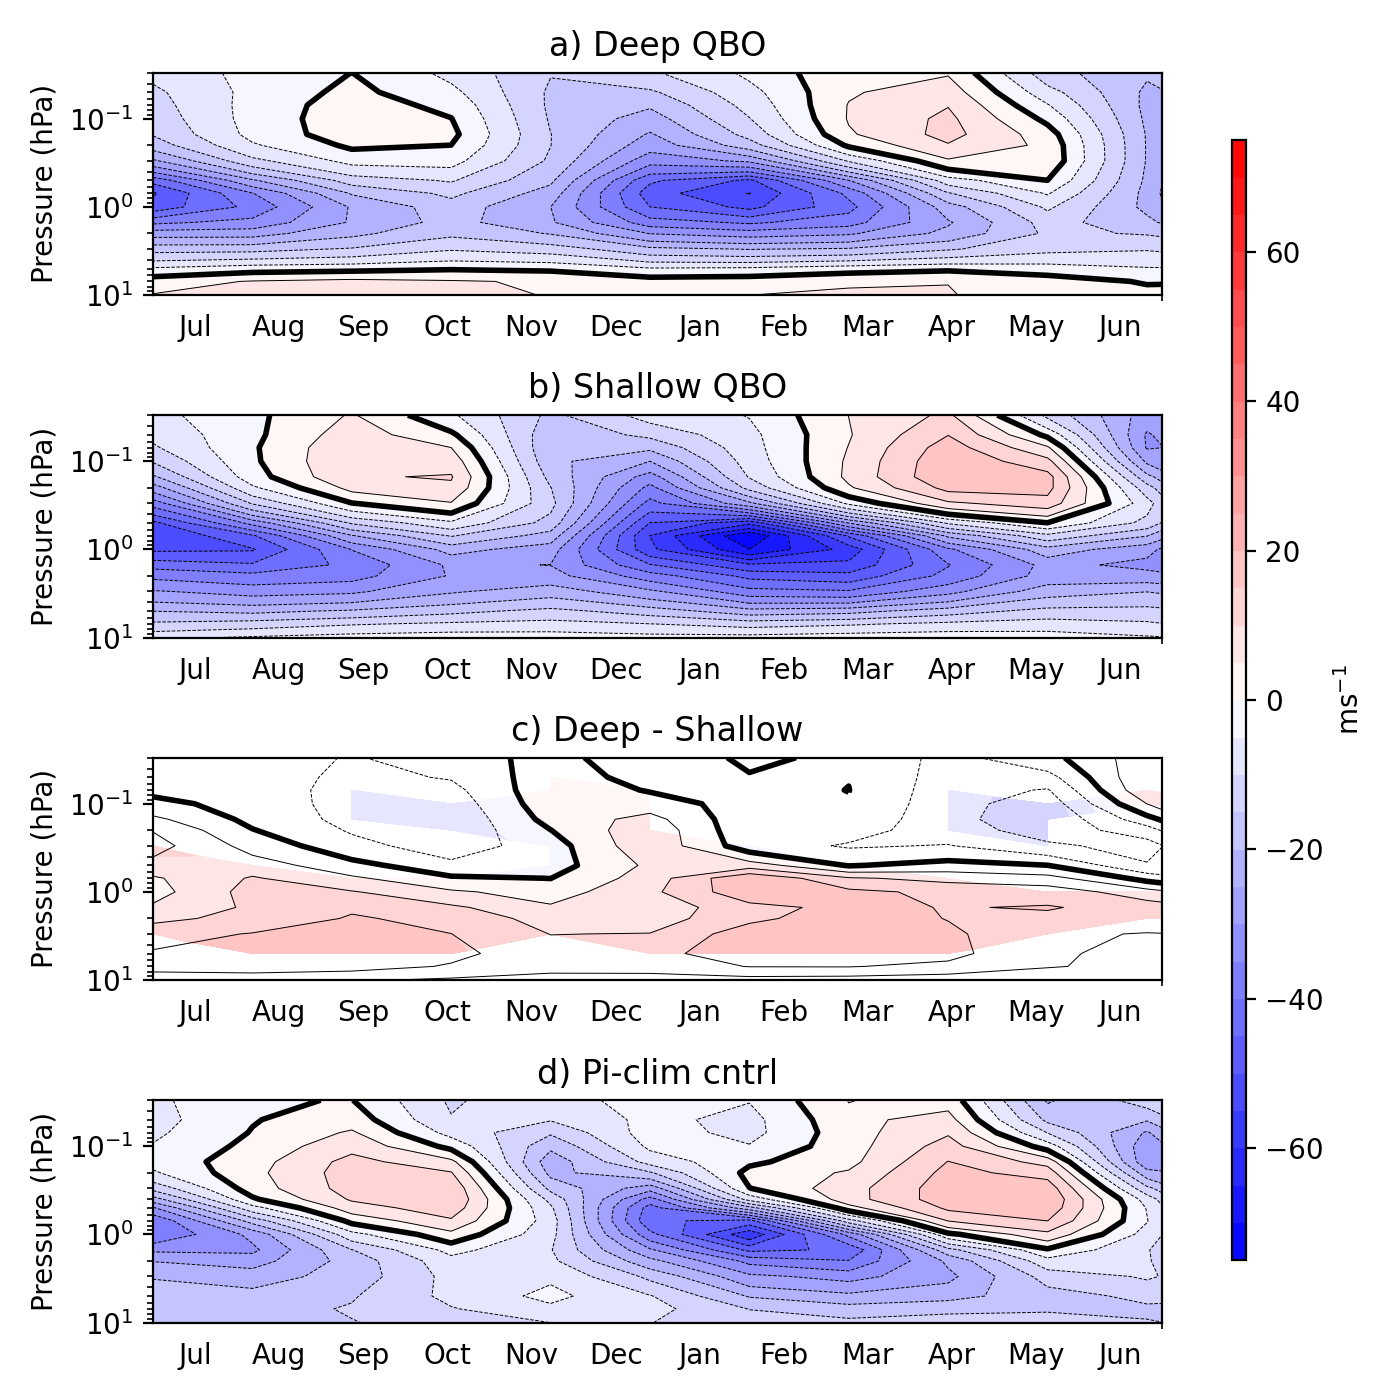
\includegraphics[width = 0.5\linewidth]{Figures/Figures-deepQBO/SAO_seasonal_cycles.png}
%\caption[Climatological seasonal cycle of equatorial ZMZW in QBO experiments]{Climatological seasonal cycle of ZMZW averaged between 5$^{\circ}$\,S--5$^{\circ}$\,N latitude from the deep (\textbf{a}) and shallow (\textbf{b}) QBO experiments. Panel \textbf{c} shows climatological differences between deep and shallow seasonal cycles. Black dots on (c) denote differences significant to the 95\% level under a 2-tailed student's t-test.}
%\label{fig:experiment_SAOs}
%\end{center}
%\end{figure}


\section{Surface responses to deep and shallow QBOs}
\label{sec:vortex_responses_QBO}
So far, we have shown that both nudged experiments exhibit the desired vertical structure in the QBO. The focus of this study however, is the different teleconnections that arise between the equatorial stratosphere and other parts of the climate system. In particular, we focus on the key finding of \cite{andrewsObserved2019d}; that the NAO and AO response to the QBO is enhanced when the QBO exhibits a higher degree of vertical coherence. 

To test this phenomenon explicitly, we analyse  diagnostics of surface variability (specifically MSLP) under different QBO conditions in the each simulation (pi-clim ctrl, deep QBO and shallow QBO) to compare the nature of teleconnections in each case. First, we examine whether the un-nudged simulation (the pi-clim cntrl) exhibits connection between the QBO and the surface. Figure \ref{fig:SLP_piclim} shows composites of NH MSLP under different QBO phases (top two rows) as well as the composite difference (QBOE-W, bottom row) for a variety of NH winter months from the deep experiment. The QBO in this plot is defined on the 50hPa level, a standard level used in previous studies and located in the middle of the nudging region for both relaxed experiments (we analyse the variation of results with QBO height in the following sections). In early winter (Nov), the response to the QBO is marginal, there is a significant positive differences in MSLP for QBOE-QBOW over the Icelandic region which corresponds to a negative NAO however this covers a relatively small region. Over mid-winter, the pattern of composite differences is difficult to recognise in terms of expected NAO/AO pattern, however responses in January exhibit negative differences over the mid-Atlantic. Overall, the responses in the un-nudged model to the QBO defined at 50hPa do not represent the expected NAO/AO pattern. This may be an indication of the model exhibiting an example of the so called "signal to noise" problem in whihc the stratospheric signal fails to significantly perturb modes of surface variation. 
%We examine whether a deep QBO metric (as used in \cite{andrewsObserved2019d}), the average equatorial winds between 15hPa and 30hPa , recovers a more coherent response. Figure 

\begin{figure}[h!]
\begin{center}
\noindent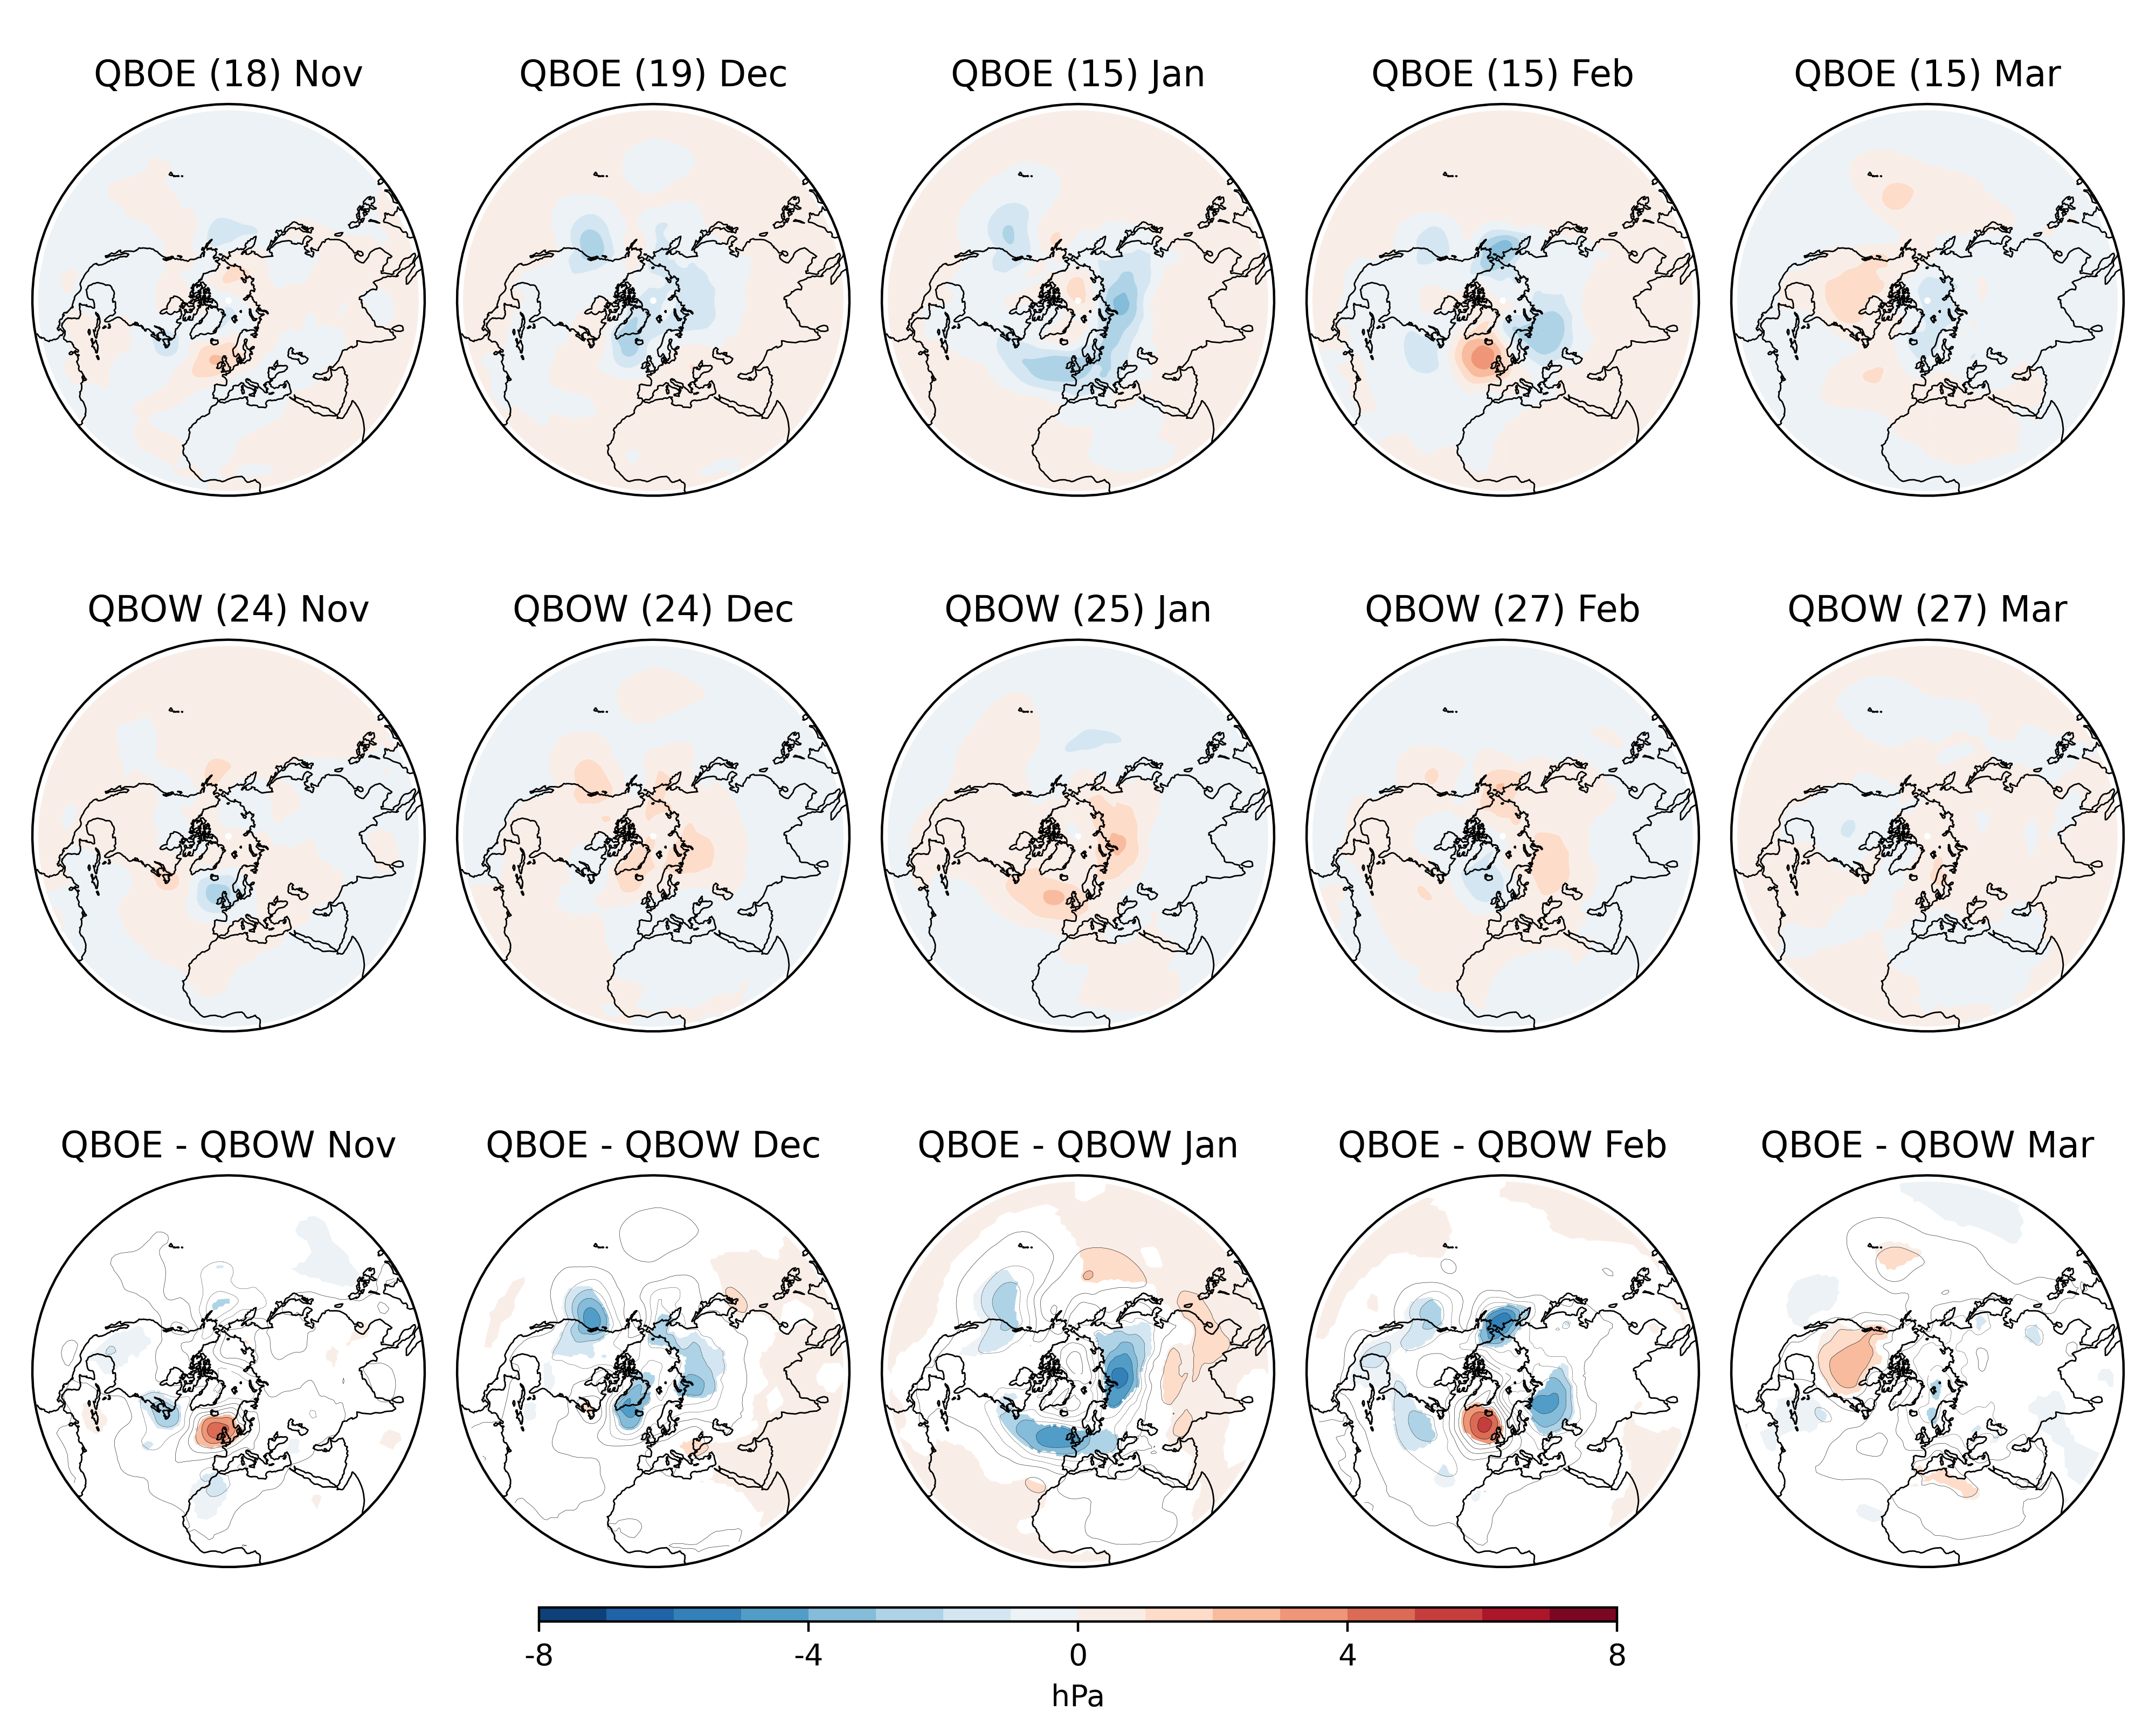
\includegraphics[width =0.8\linewidth]{Figures/Figures-deepQBO/SLP_composites_individual_months_QBO_phases_U_piclim_30hPa_5thresh.png}
\caption[]{NH deseasonalised MSLP anomaly composites for the QBO East (top row), QBO West (middle row) phases and composite differences (QBOE - QBOW, bottom row) for the pi-clim cntrl simulation. The QBO phase is defined as any monthly equatorial ($5^{\circ}$\ S--$5^{\circ}\ $N average) ZMZW that exceeds a magnitude of 5\ m\,s$^{-1}$ on the 50hPa level in various months (which are indicated in sub-figure titles). Numbers in parentheses indicate the number of winters of each phase that make up the composite. Coloured shading in the bottom row indicates MSLP differences significant above the 95\% confidence level under a 2 tail student’s t-test.}
\label{fig:SLP_piclim}
\end{center}
\end{figure}

In contrast, the deep QBO experiment MSLP composites (figure \ref{fig:SLP_deep}) exhibits a prominent signal in the NAO region indicated by a composite difference of up to 8hPa which is significant under a t-test. This signal is most apparent in mid-late winter (Jan-Mar), although a similar anomaly is visible in November. This feature corresponds to positive (negative) MSLP anomalies under QBOE (QBOW) conditions centred over the southern node of the NAO (a region encompassing the Azores) indicating that it may originates through the sub-tropical pathway discussed in \cite{graySurface2018b} as opposed to via modulation of the vortex which exhibits greater association with the northern node of the NAO (ref? xxxxx) however this requires further diagnostics to understand fully (see the following section). Indeed, these patterns indicate a shift towards a positive NAO pattern under QBOE conditions and negative NAO under QBOW - the opposite sign to a response expected via a Holton-Tan mechanism which would predict a weakened (strengthened) vortex and subsequent negative (positive) NAO under QBOE (QBOW) phases. Furthermore, \cite{andrewsObserved2019d} show a response consistent with a Holton-Tan link and of the opposite sign to those shown here (positive NAO phase under QBOW conditions) using their deep QBO metric so these results are somewhat surprising and warrant further study into their origins which is presented in the following sections.

\begin{figure}[h!]
\begin{center}
\noindent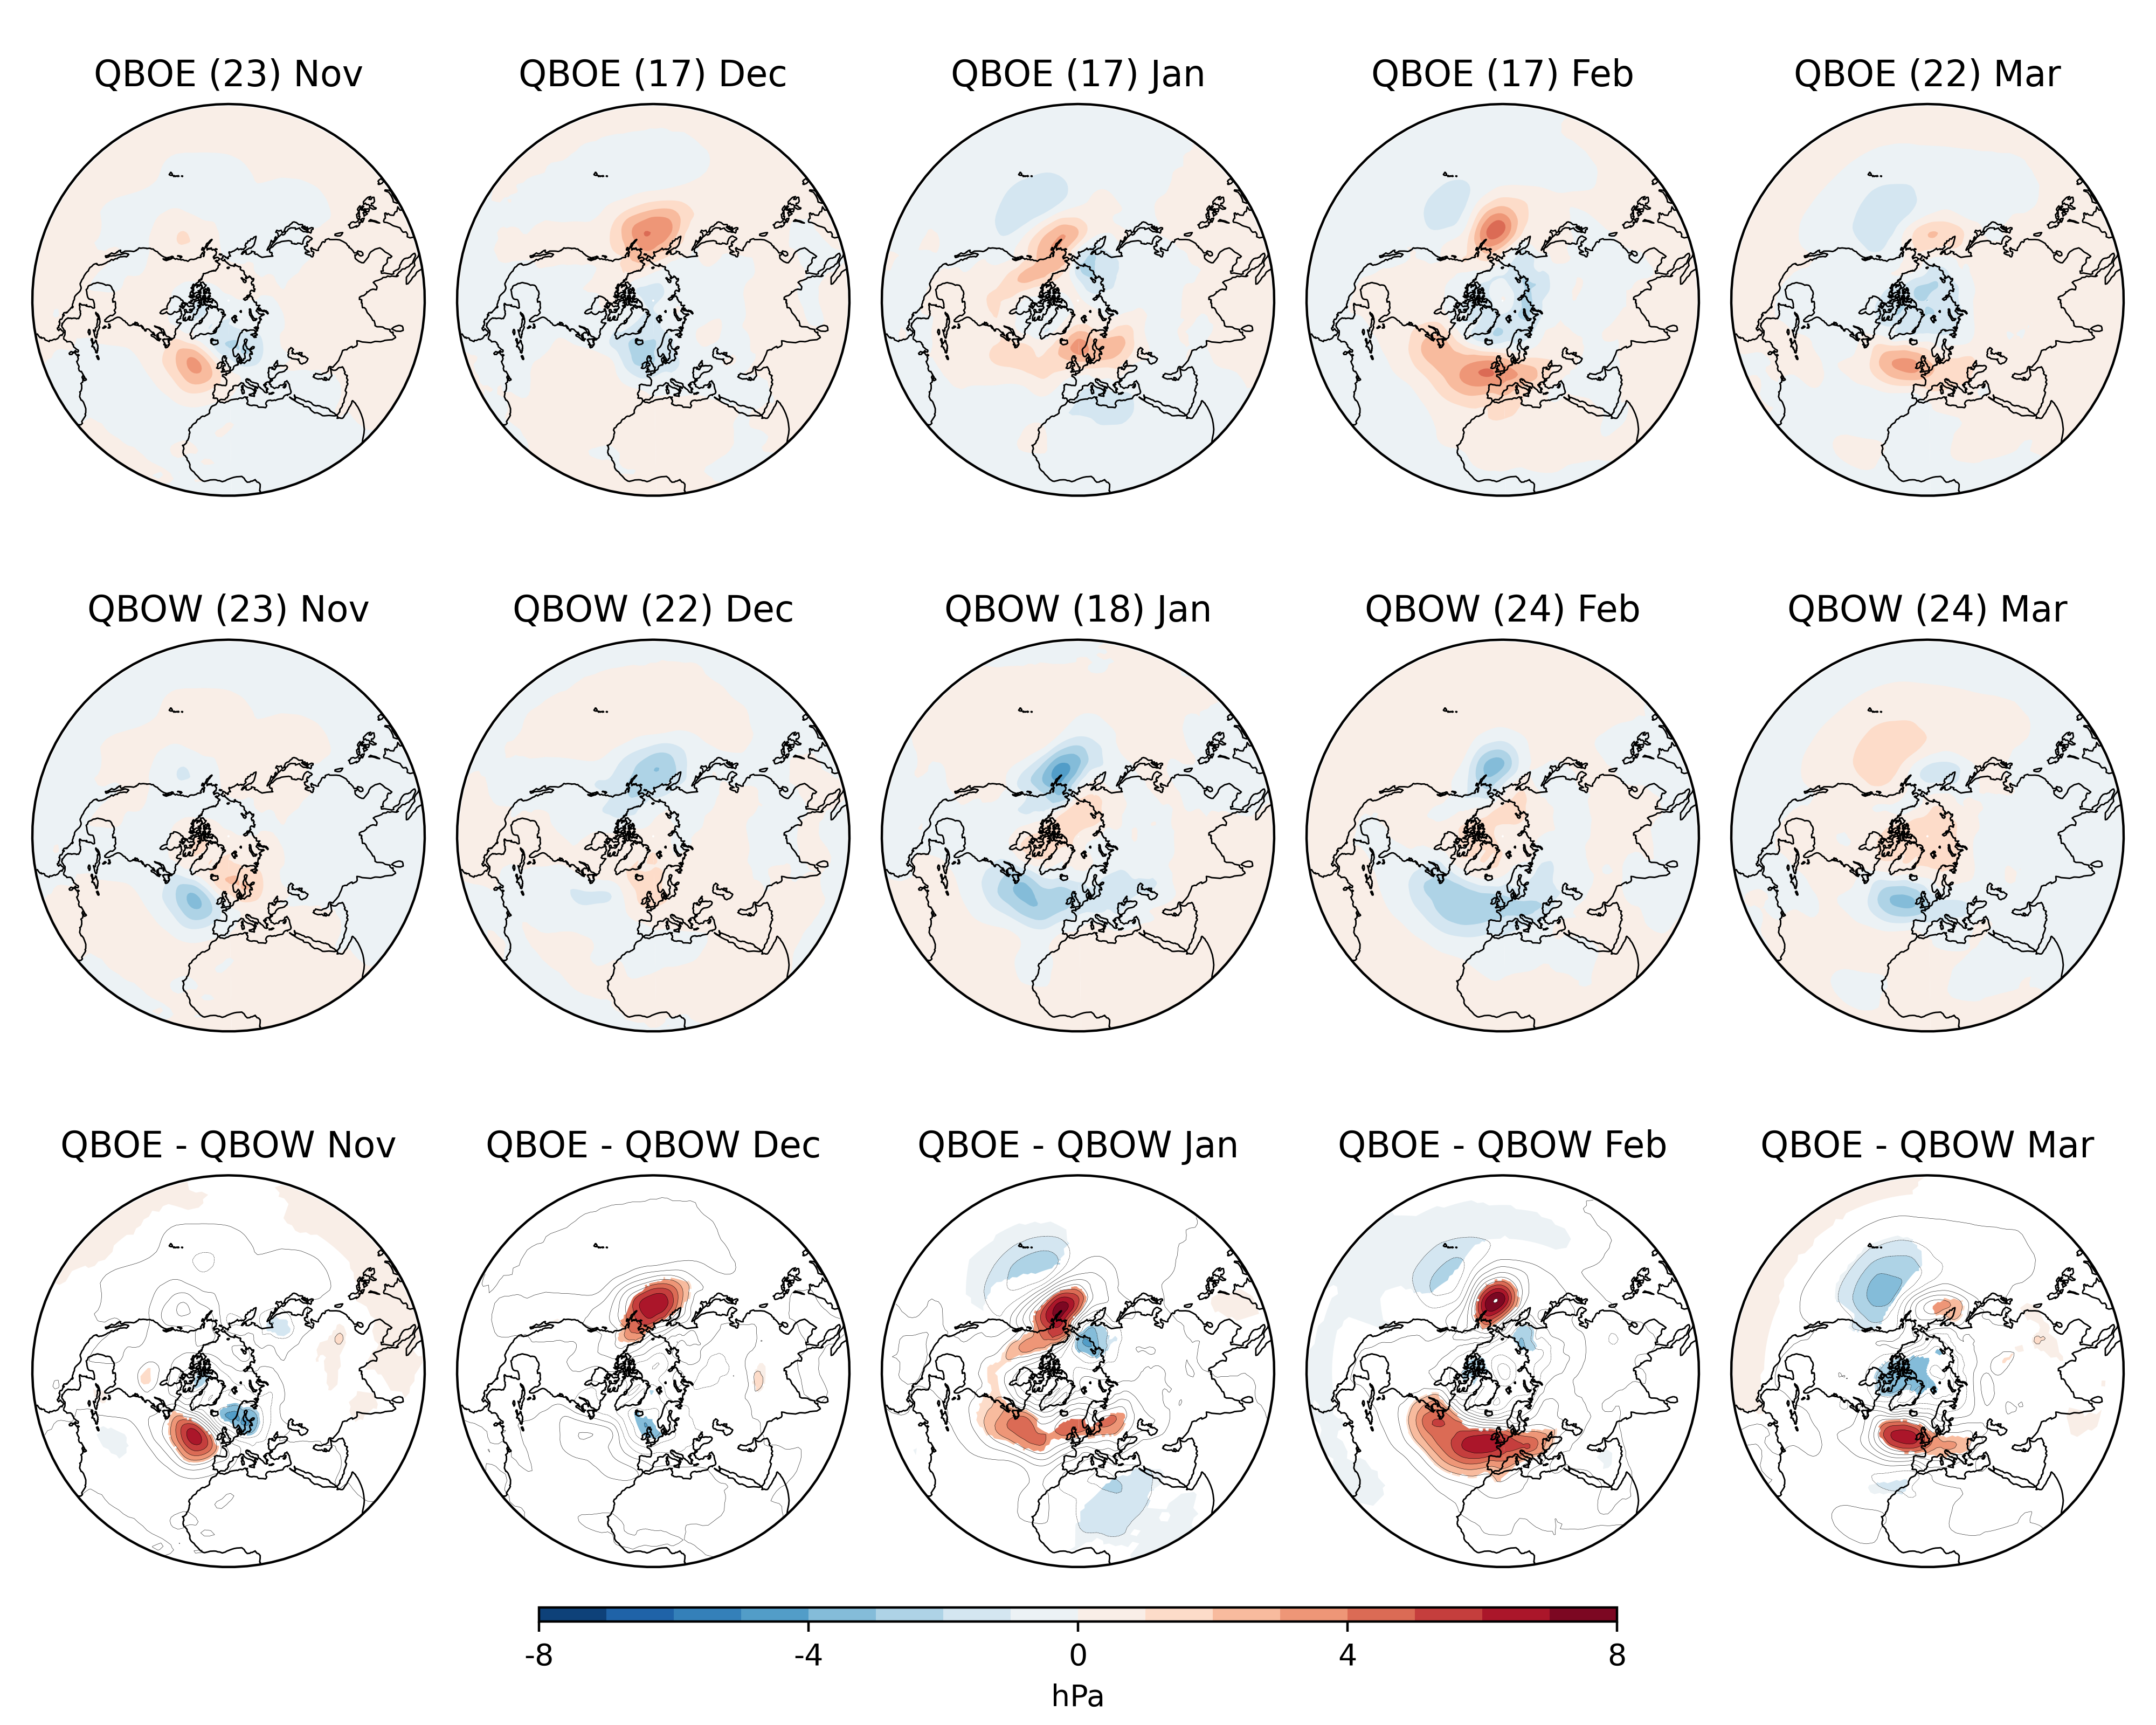
\includegraphics[width =0.8\linewidth]{Figures/Figures-deepQBO/SLP_composites_individual_months_QBO_phases_U_d_higher_50hPa_5thresh.png}
\caption[]{Like figure \ref{fig:SLP_piclim} for the deep QBO experiment.}
\label{fig:SLP_deep}
\end{center}
\end{figure}

The corresponding Atlantic responses from the shallow QBO experiment (figure \ref{fig:SLP_shallow}) are markedly different to its deep counterpart: The magnitude of responses to individual QBO phases (top two rows) as well as differences (bottom row) are smaller than in the deep experiment (gives maxima here xxxxx) and a smaller region of composite differences are deemed significant under a 2 tailed t-test (also bottom row). This result is consistent with the primary findings of \cite{andrewsObserved2019d} who report an enhanced NAO response to a deep QBO metric compared to a single level QBO index (although the responses shown for our experiments are of the opposite sign). There is also greater intra-seasonal variability in the response patterns' structure with negative composite differences in early winter (Nov-Jan) over the east Atlantic for November and the Icelandic node of the NAO for December and January. In late winter (Mar) positive composite differences are prominent over the Azores node of the NAO. 

There is also a MSLP response in the North Pacific in both nudged experiments concentrated over the AL region which corresponds to the Pacific node of the AO (see figure \ref{fig:AO}). As with the Atlantic response, the deep experiment exhibits anomalies with larger amplitude than the those in the shallow, a finding also consistent with \cite{andrewsObserved2019d}. Both experiments' Pacific responses are most prominent in mid NH winter (Dec-Feb) consistent with similar findings in \cite{graySurface2018b} that show significant anomalies over this region peak in February. The sign of the anomalies in this region for both experiments indicate that a positive (negative) pacific pattern corresponds to QBOE (QBOW) conditions, an influence which is likely due to the subtropical pathway as d
iscussed in \cite{graySurface2018b}. Overall, results comparing MSLP composites in our two nudged experiments indicate enhanced response patterns to a perpetually deep QBO consistent with the results from previous studies \citep{graySurface2018b, andrewsObserved2019d} and possibly suggesting the importance of vertical structure in teleconnections. However, the Atlantic response in the deep experiment is of the opposite sign to the expected HT mechanism and therefore a closer examination of possible pathways involved in this response is required to understand the importance of vertical coherence in the QBO.

\begin{figure}[h!]
\begin{center}
\noindent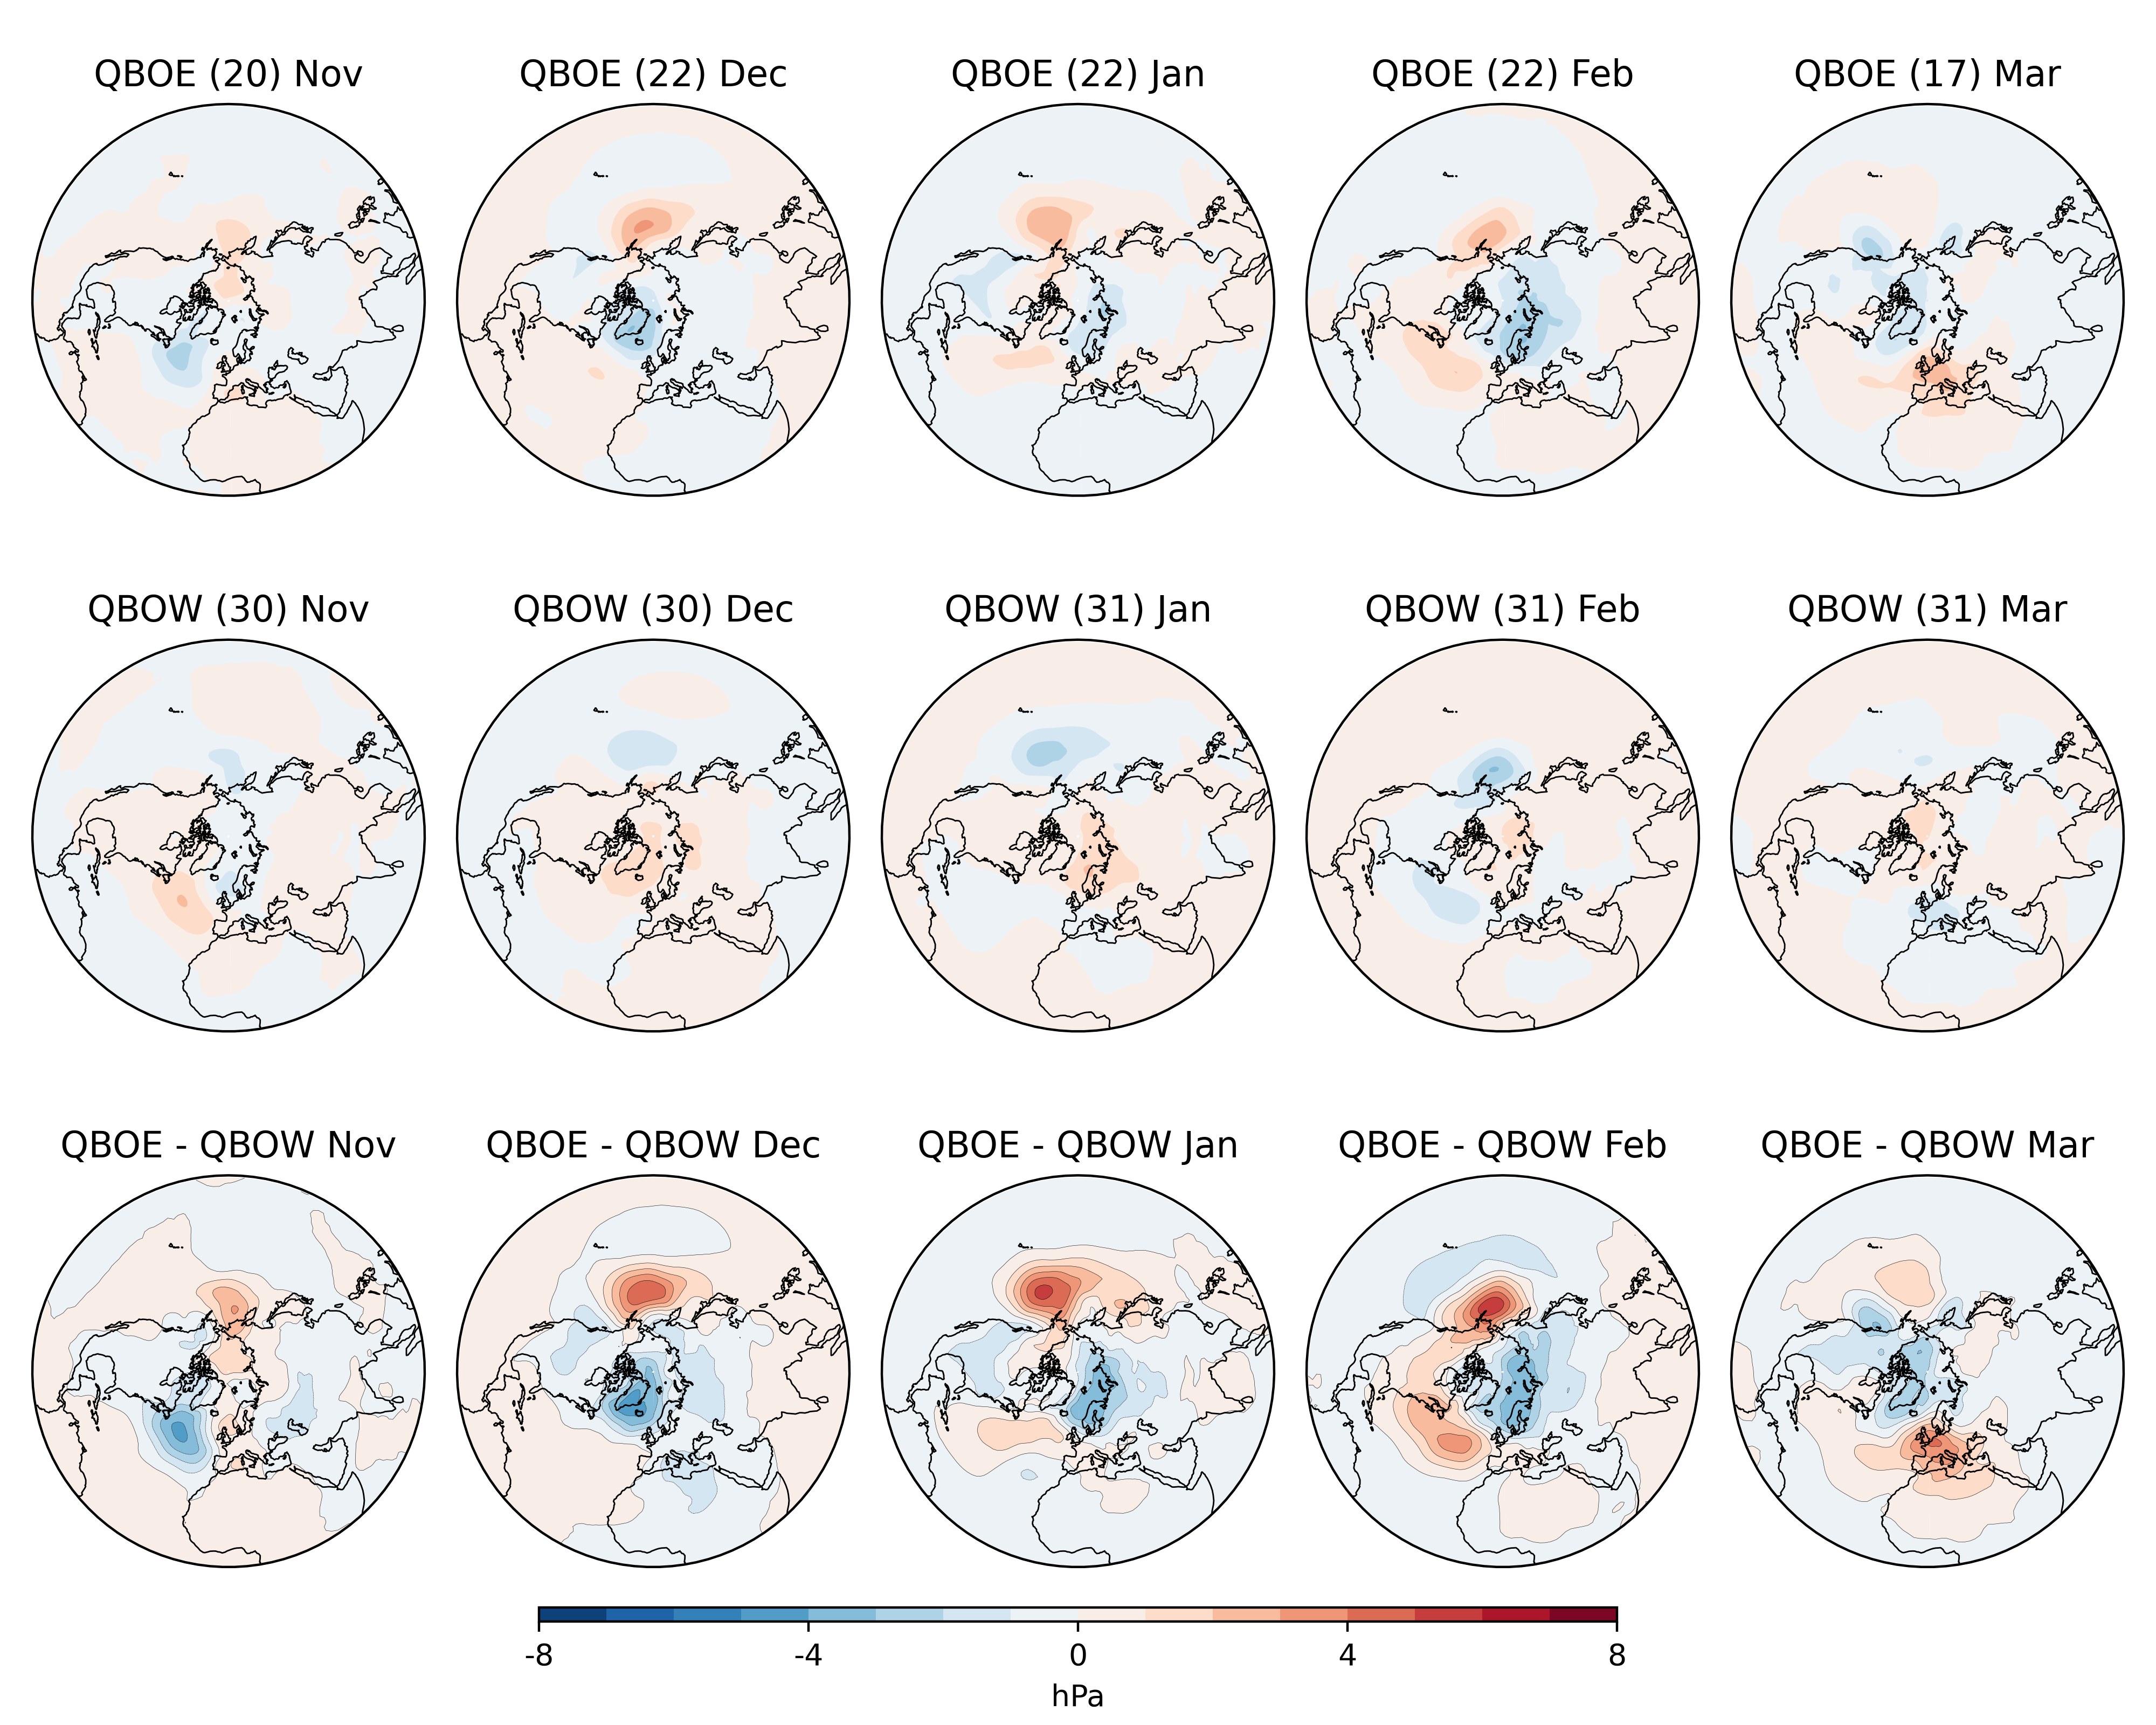
\includegraphics[width =0.8\linewidth]{Figures/Figures-deepQBO/SLP_composites_individual_months_QBO_phases_U_s_50hPa_5thresh.png}
\caption[]{Like figure \ref{fig:SLP_piclim} for the shallow QBO experiment.}
\label{fig:SLP_shallow}
\end{center}
\end{figure}
\newpage

\section{Vortex responses to the QBO}
The surface responses to QBO phases presented in figures \ref{fig:SLP_deep} and \ref{fig:SLP_shallow} suggest that surface signals associated with the QBO may be enhanced with a vertically coherent QBO. However, the pathways involved are not well understood and the late winter anomalies in the Atlantic region are of the opposite sign to an expected HT effect and not fully explained.

We next analyse the interaction between the QBO and the vortex in each experiment to further understand the possible mechanisms involved in the surface responses seen in the previous section. Figure \ref{fig:HT_deep} shows a measure of the strength of the Holton-Tan effect in the pi-clim cntrl simulation -  composite differences between NH winter ZMZW under QBOE and QBOW conditions (QBOE-QBOW) defined on various pressure levels (columns in figure \ref{fig:HT_piclim}) and for a range of NH winter months (rows). The response from the vortex in this un-nudged simulation broadly reflects the composites from the fully coupled pi-control simulation of UKESM (figure \ref{fig:holton_tan_comp}) with negative composite differences in the vortex for QBOE-QBOW conditions defined on the 20hPa and 30hPa levels. This is consistent with the HT effect discussed in section \ref{sec:external_influence_HT} in which the easterly QBO phase induces a weakened vortex (see figure \ref{fig:HT_piclim}, left column). The majority of these negative differences are concentrated in early-mid winter months (Nov-Jan), a finding also reported in \cite{graySurface2018b}. There are marginal negative composite differences to the QBO at 70hPa and 50hPa also in early winter which extend to 50N (while winds at 60N is normally used as a measure of the vortex edge). In late winter (Feb-Mar), the response of the vortex reduces and even reverse to positive on the 70hPa level (again, an effect reported in \cite{graySurface2018b}). These composites indicate that the un-nudged configuration of the model is able to reproduce a clear coupling between the QBO and the vortex suggesting the suitability of this model configuration for QBO-vortex analysis with nudged QBO simulations.

The corresponding ZMZW composite differences between QBO phases in the deep and shallow experiment (figure \ref{fig:HT_deep} and \ref{fig:HT_shallow} respectively) show distinct response patterns. In early winter (November), both simulations exhibit negative composite differences in the vortex for QBOE - QBOW conditions, consistent with a HT mechanism \citep{holtonNumerical1980} as well a the pi-clim cntrl (figure \ref{fig:HT_piclim}). The magnitude of vortex responses in early winter months is marginally larger in the deep experiment compared to that of the shallow and pi-clim cntrl and deep responses are present for all sampled pressure levels while the shallow and pi-clim cntrl responses show some variation with QBO pressure level. 

\newpage
\begin{figure}[h!]
\begin{center}
\noindent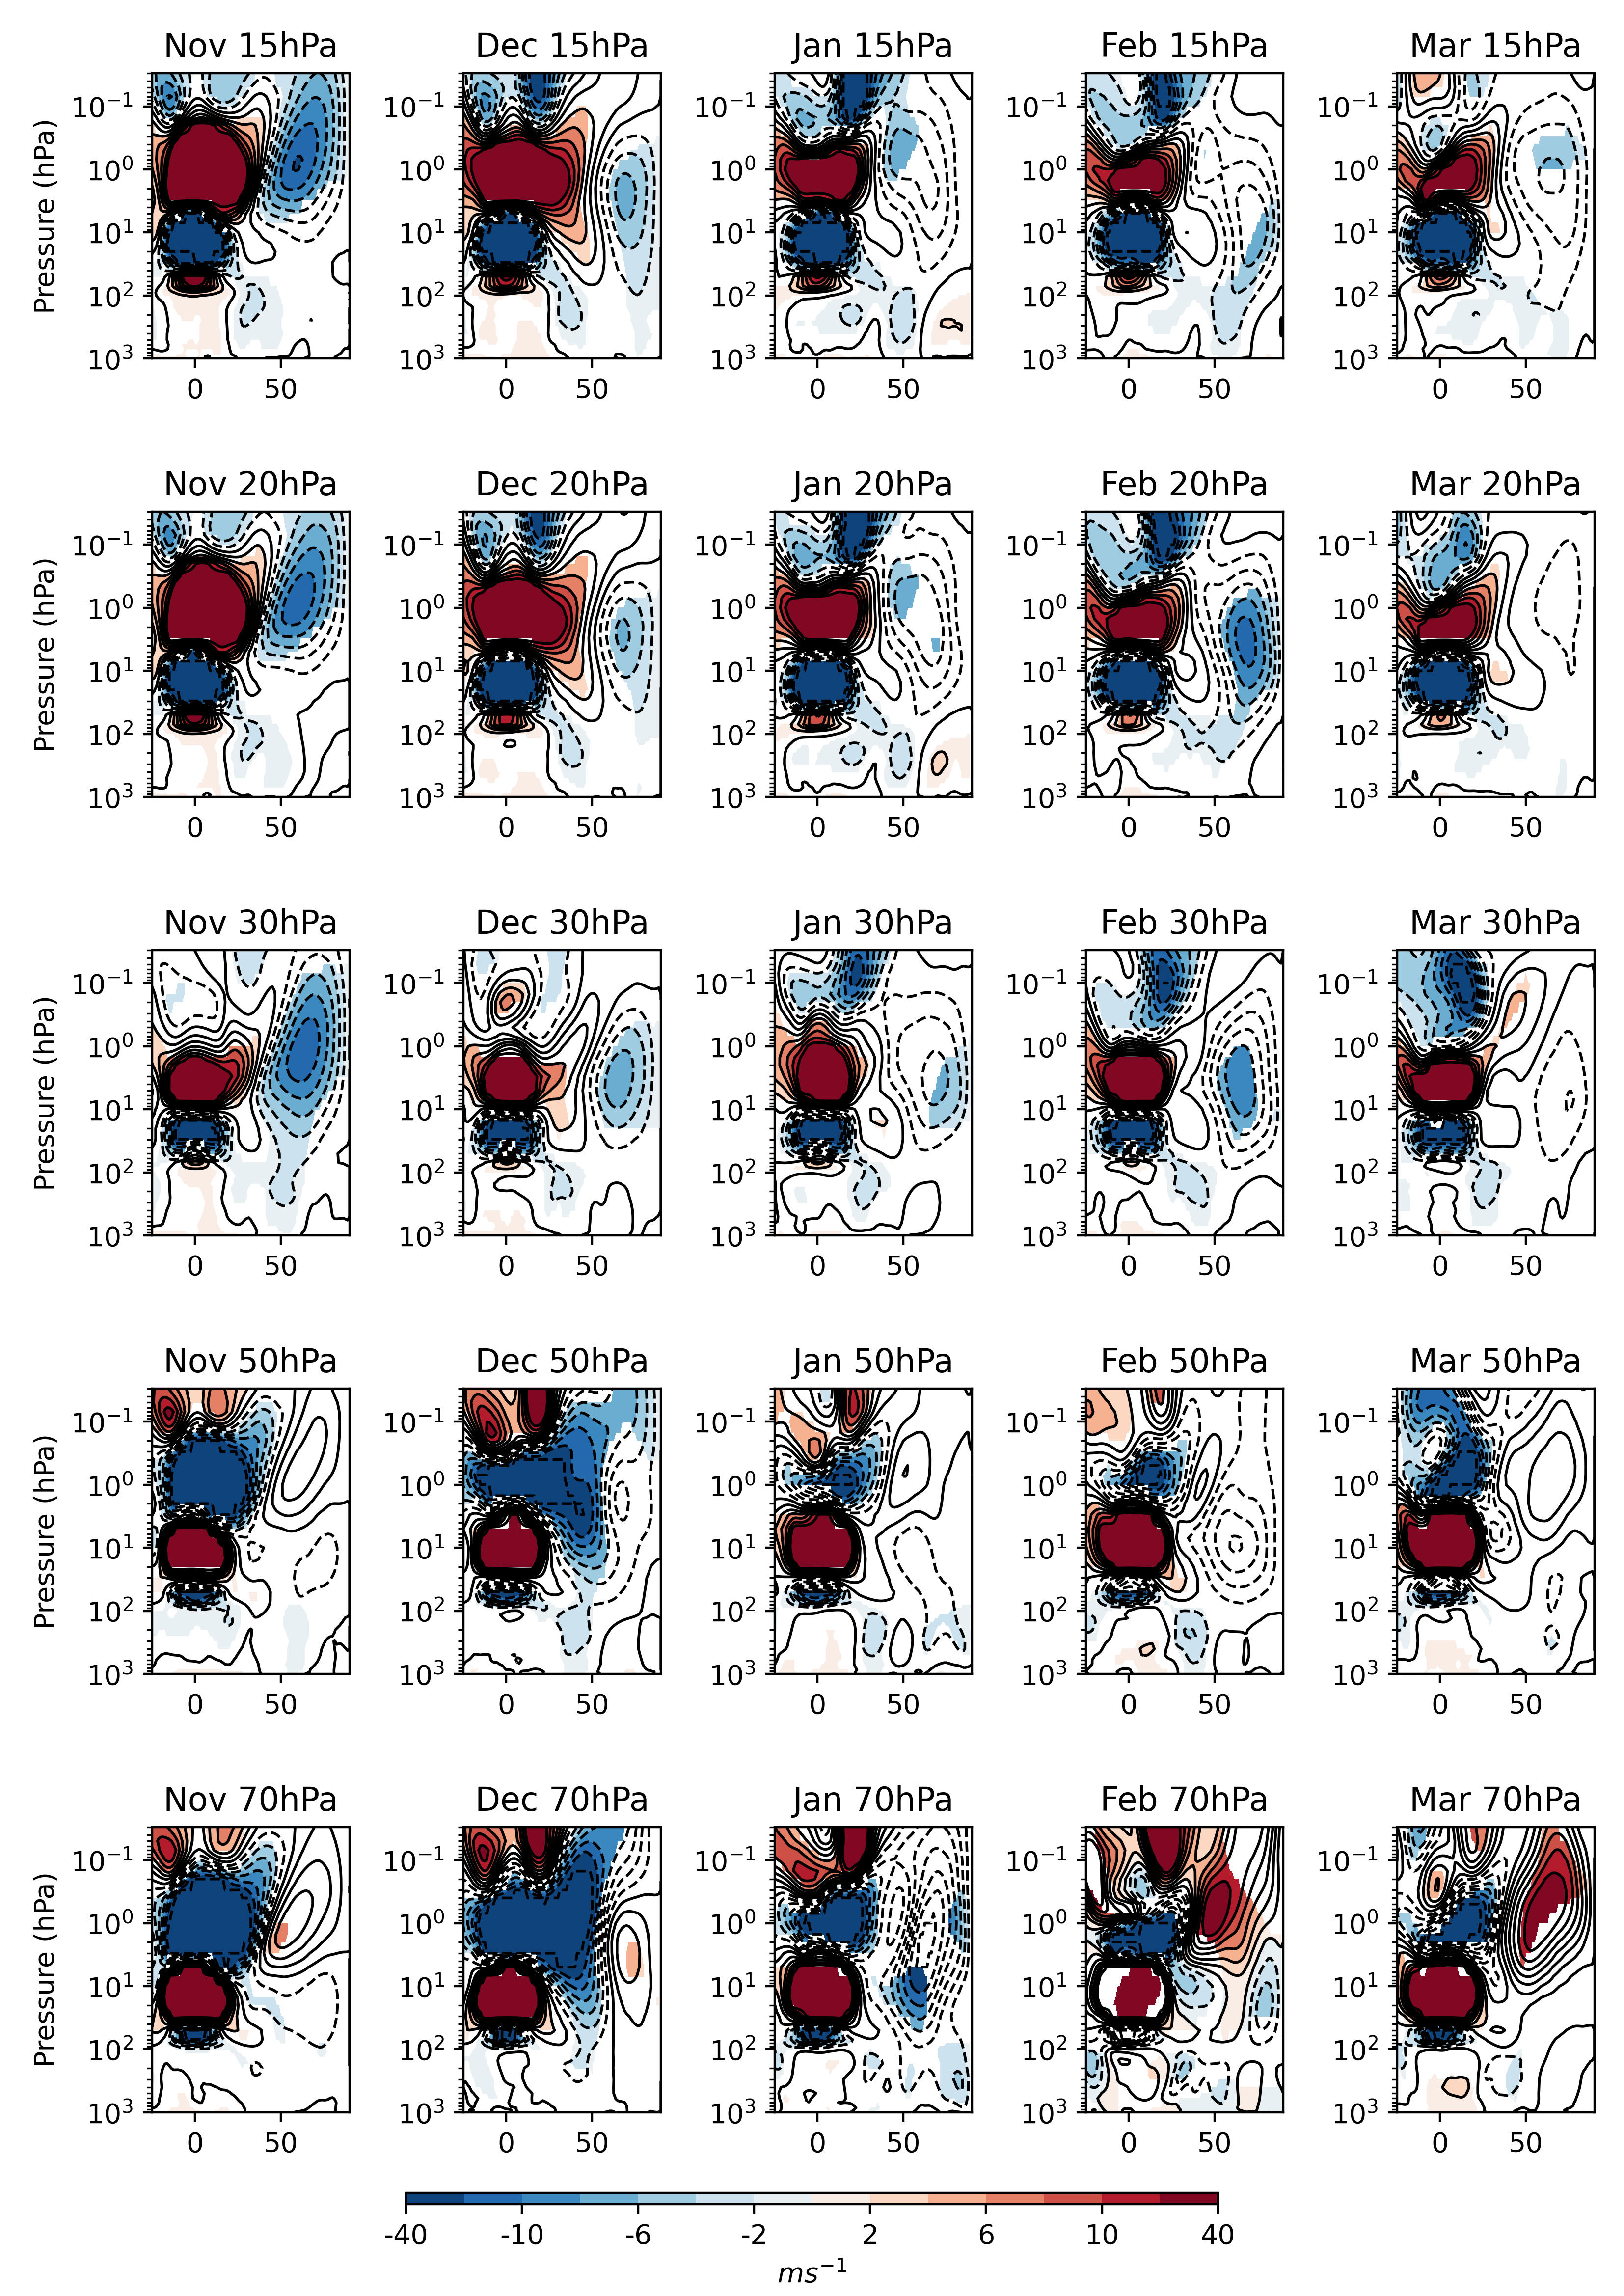
\includegraphics[width = 0.9\linewidth]{Figures/Figures-deepQBO/ZMZW_composites_by_month_QBO_phases_U_piclim_MarQBO_vs_Mar_70hPa_5thresh.png}
\caption[]{}
\label{fig:HT_piclim}
\end{center}
\end{figure}
\newpage

\begin{figure}[h!]
\begin{center}
\noindent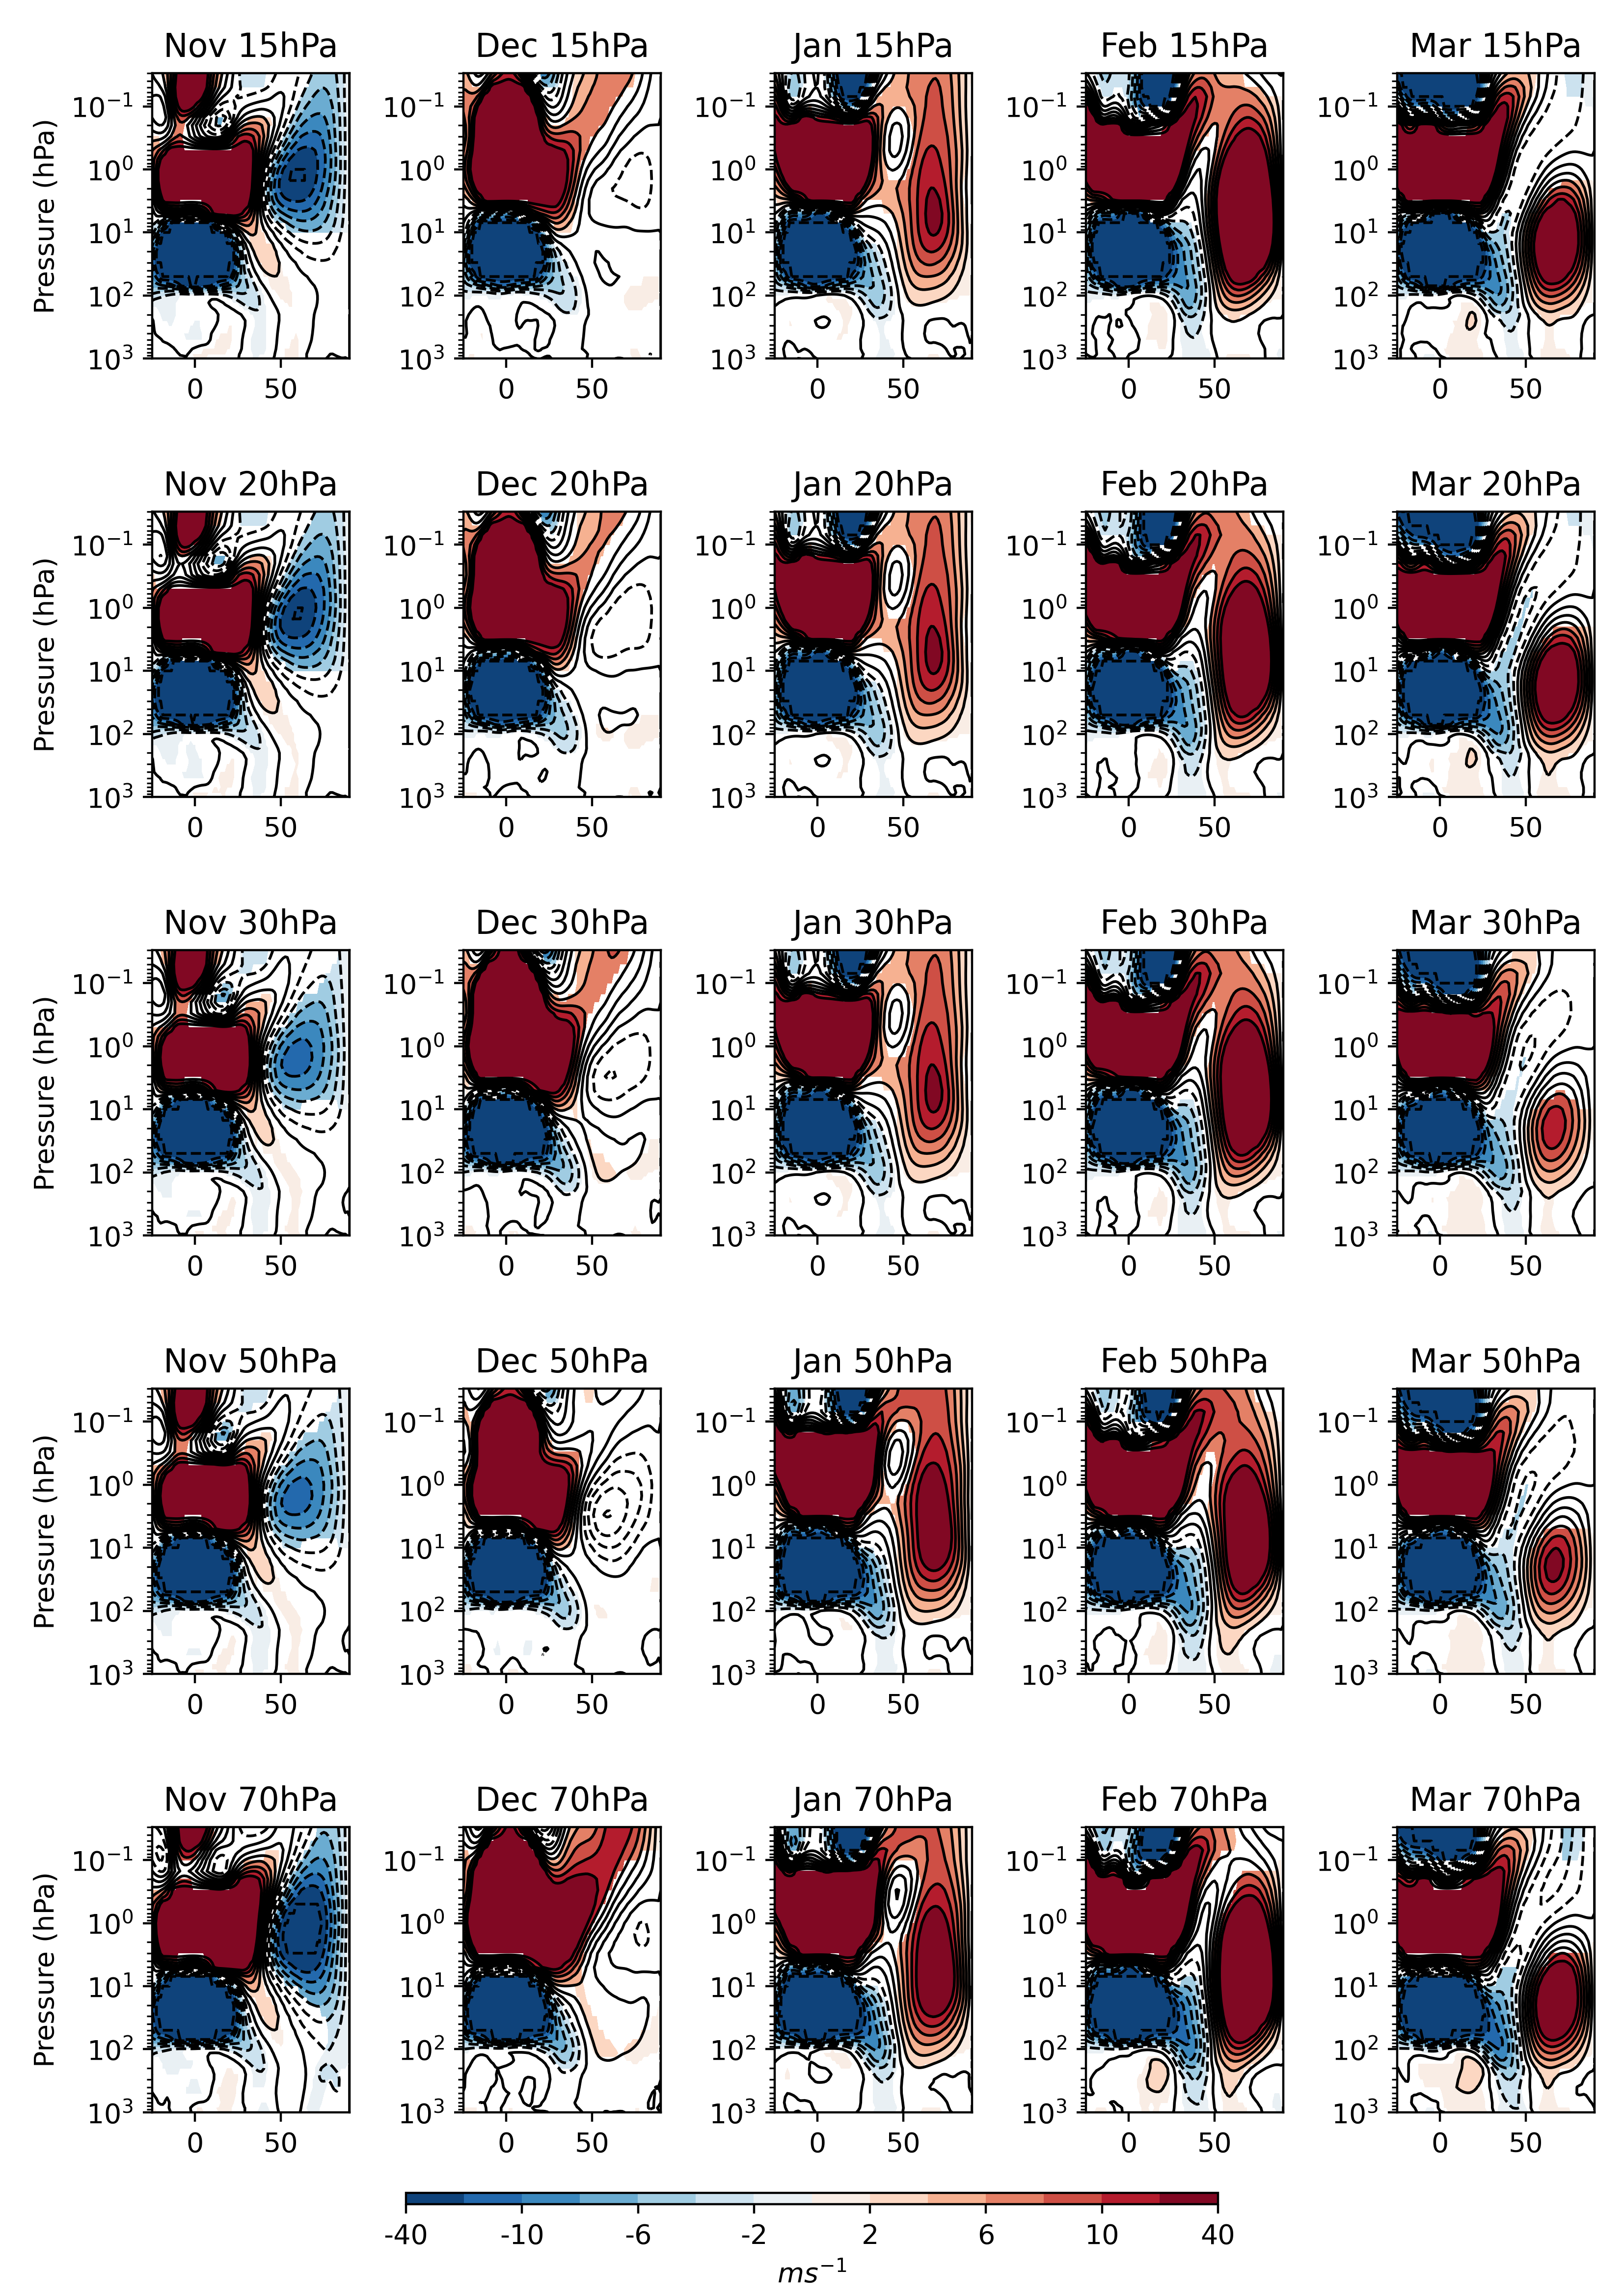
\includegraphics[width = 0.9\linewidth]{Figures/Figures-deepQBO/ZMZW_composites_by_month_QBO_phases_U_d_higher_MarQBO_vs_Mar_70hPa_5thresh.png}
\caption[]{Like figure \ref{fig:HT_piclim} for the deep experiment}
\label{fig:HT_deep}
\end{center}
\end{figure}

\begin{figure}[h!]
\begin{center}
\noindent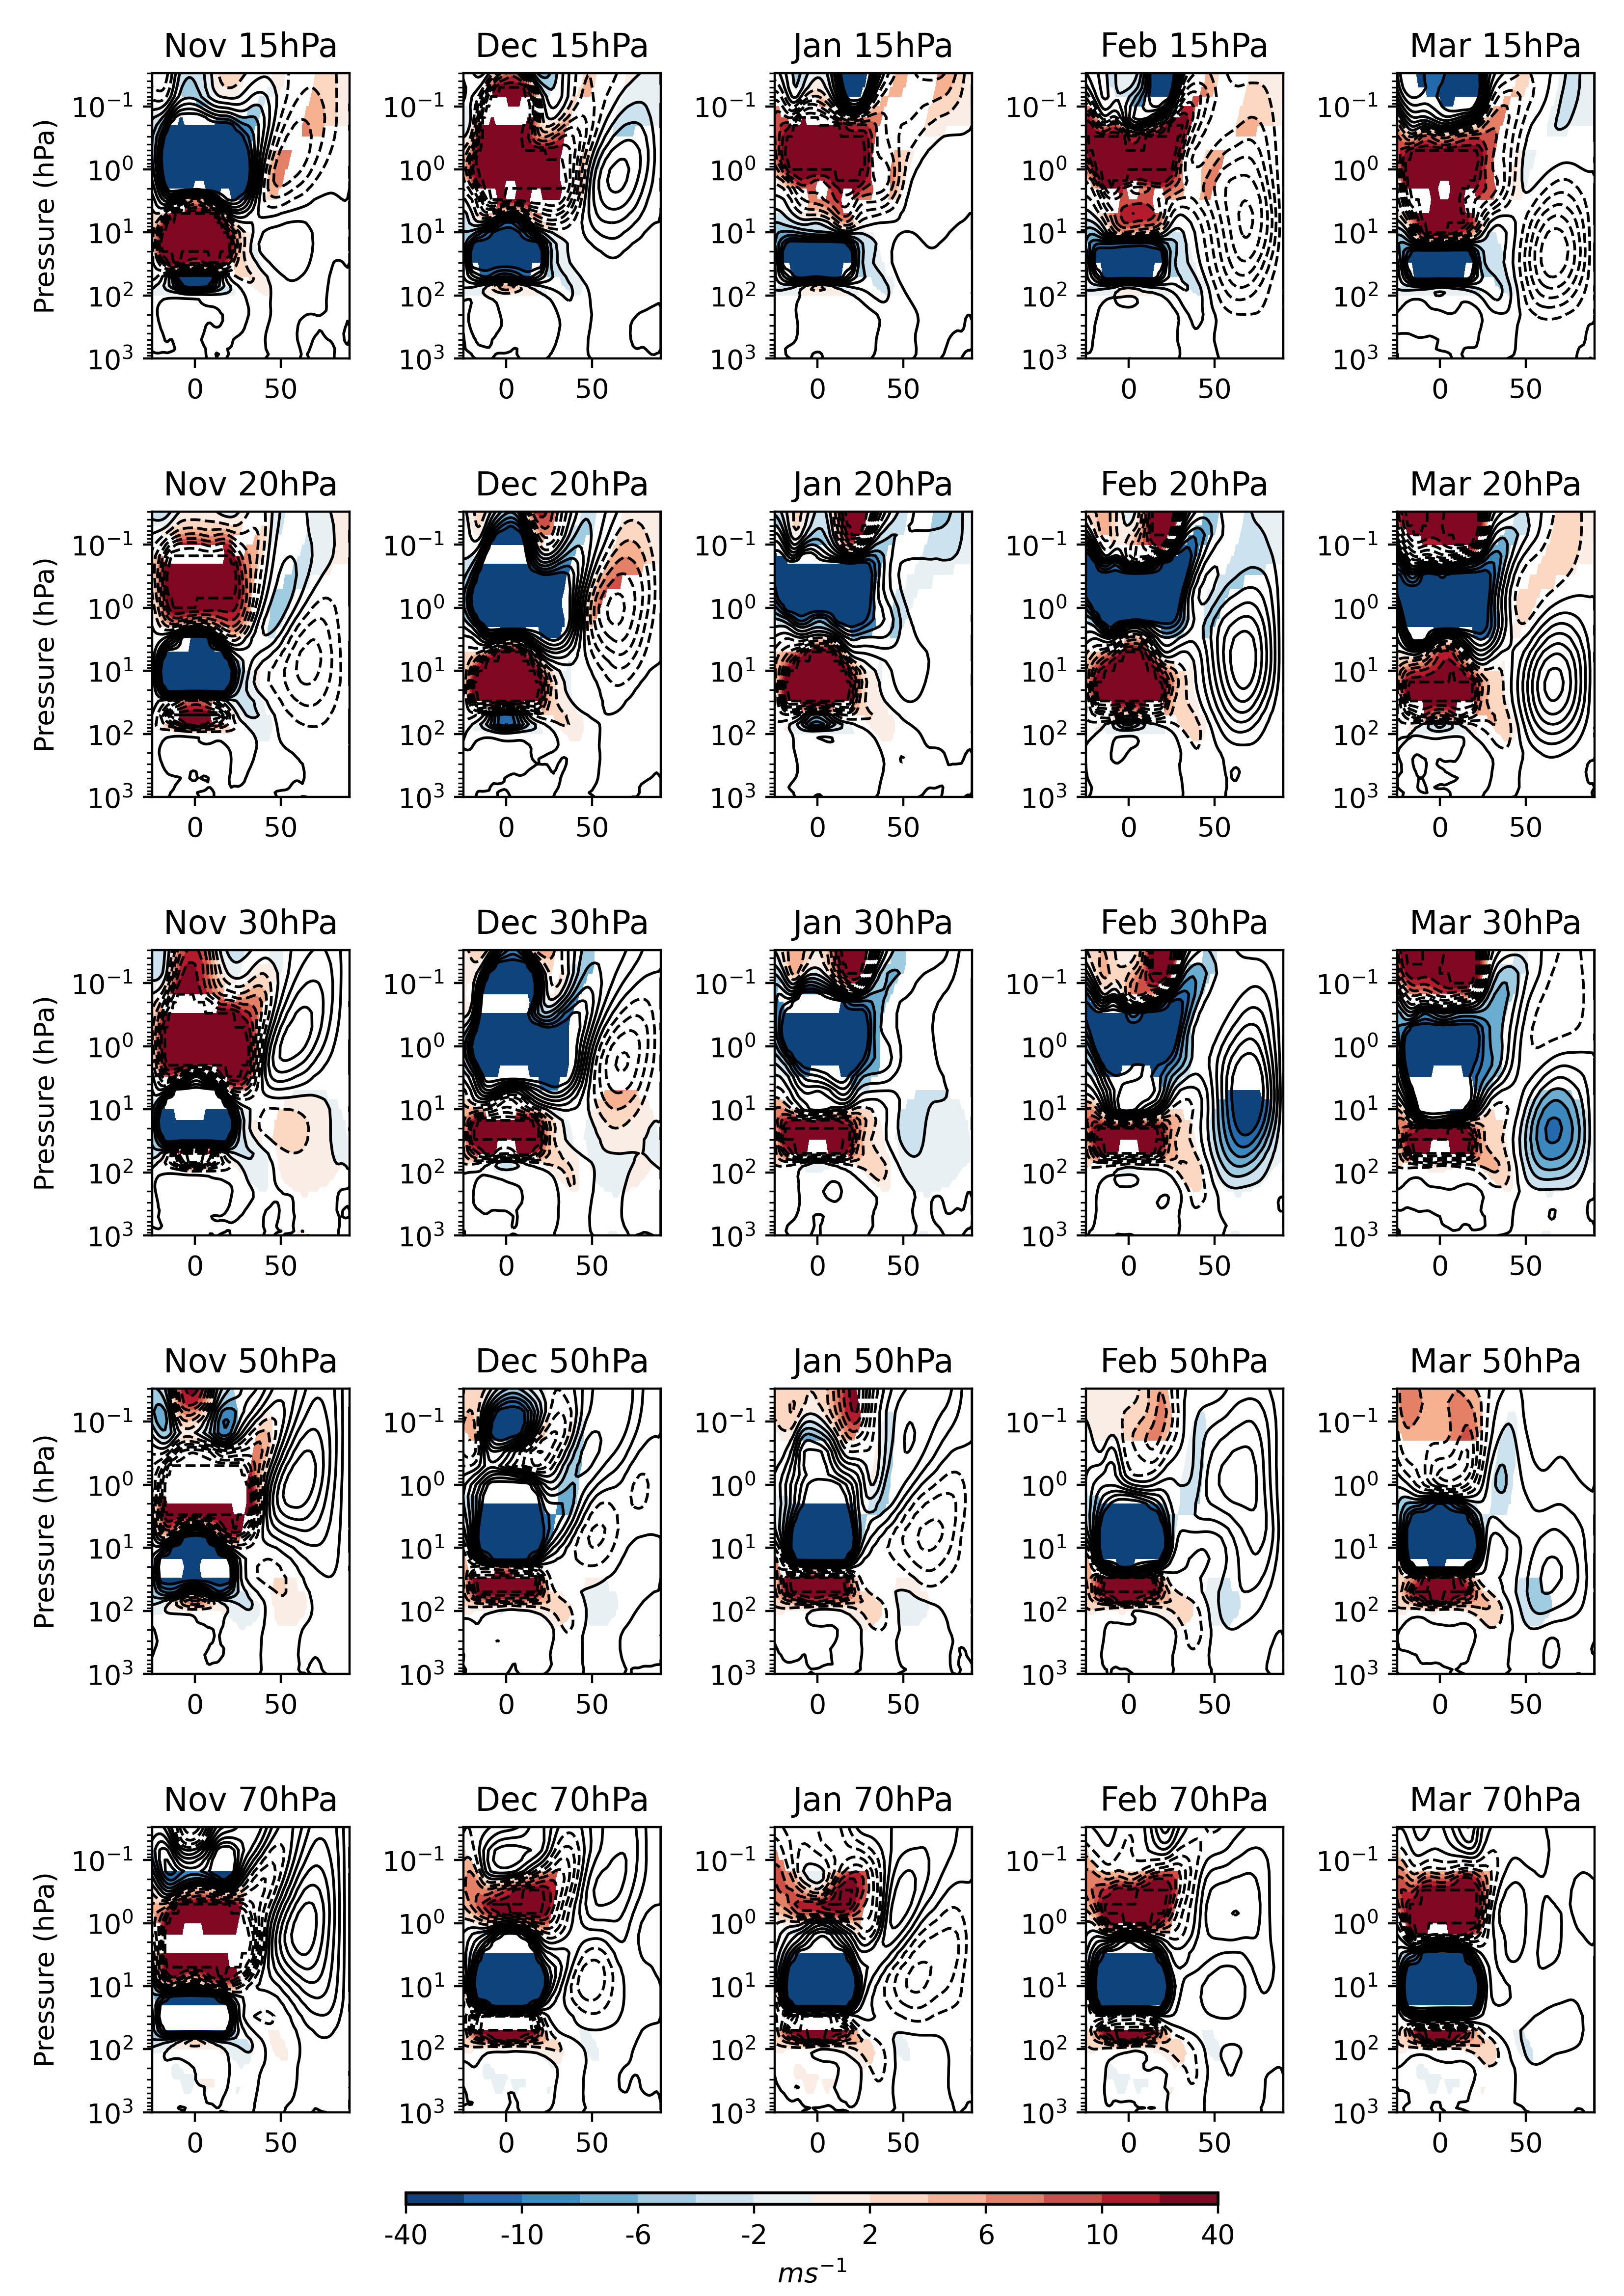
\includegraphics[width = 0.9\linewidth]{Figures/Figures-deepQBO/ZMZW_composites_by_month_QBO_phases_U_s_MarQBO_vs_Mar_70hPa_5thresh.png}
\caption[]{Like figure \ref{fig:HT_piclim} for the shallow QBO experiment.}
\label{fig:HT_shallow}
\end{center}
\end{figure}
\newpage 

In mid-late winter (Jan-Mar) the deep experiment exhibits remarkably large positive composite differences of the vortex (up to xxxx $ms^{-1}$). This notable feature is largely absent in the pi-clim cntrl (figure \ref{fig:HT_piclim}) as well as the shallow experiment (figure \ref{fig:HT_shallow}) and may point to an enhanced vortex response in the deep experiment compared to other simulations. There is a response to the QBO at 30hPa in the shallow experiment with positive differences evident for February and March but these are significantly smaller in magnitude than those in the deep QBO simulation. These positive differences in the deep experiment are of the opposite sign to the expected HT relation however they do reflect some results in \cite{graySurface2018b} who demonstrate an seasonal progression between early and later NH winter in QBO-vortex interactions. They may also account for the positive (negative) NAO pattern MSLP responses to QBOE (QBOW) in late NH winter in figure \ref{fig:SLP_deep}; in these months the vortex appears strengthened (weakened) under QBOE (QBOW) conditions which may in turn induce a positive (negative) NAO through the vortex's in-season influence over the NAO \citep{charlton-perezInfluence2018e}. 

Also evident in the ZMZW composites from the deep experiment (figure \ref{fig:HT_deep}) are elements of connection between the QBO and the surface: Between xxx-xxx latitudes, a limb of anomalies associated with QBO phases descends into the troposphere (below 100hPa) and to the surface. These anomalies are of the same sign as the QBO anomaly in the middle equatorial stratosphere and increases in magnitude as well as propagation towards the surface throughout the winter season with significant composite differences reaching the surface in February and March. This feature is not evident in the composites of the shallow experiment but is observed in the pi-clim cntrl albeit at a lower magnitude and only for a selection of months (February and March using a 30hPa QBO, for example). This feature may be evidence in support of a subtropical pathway between the QBO and surface suggested in \cite{graySurface2018b} as one of the mechanisms by which the QBO exerts influence over surface variability. It also appears to be heavily enhanced by the presence of a vertically coherent QBO. This pathway is studied in further detail in section xxxxxx. 

\section{The role of the SAO}
ZMZW composites in figures \ref{fig:HT_piclim}-\ref{fig:HT_shallow} showed positive (negative) vortex responses to QBOE (QBOW) conditions in late winter which are significantly enhanced in the deep experiment compared to the shallow and pi-clim cntrl simulations and may be responsible for the enhanced late winter MSLP response (figure \ref{fig:SLP_deep}). However, the cause of these large responses in the vortex are as yet to explained and understanding this feature further may be key in diagnosing the role of a deep QBO in surface teleconnections.

A prominent feature of the ZMZW composites in the deep simulation (figure \ref{fig:HT_deep}) is the SAO region (above the 1hPa level): Composite differences in the upper equatorial stratosphere in this experiment exhibit large anomalies of the opposite sign of the QBO phase below. These anomalies are evident throughout NH winter season are not sensitive to the choice of QBO level. This is consistent with the idea of vertically coherent QBO phases filtering out waves with the same phase speed direction as the QBO and permitting wave forcing of the opposite phase speed into the lower mesosphere leading to anomalies of the opposite sign (ref here). There is some suggestion of similar SAO anomalies in the shallow experiment but they are smaller in magnitude than in the deep QBO experiment, not present for composite differences on all levels (minimal SAO signal is apparent for 50hPa composites) and are more confined to the equatorial region.

There is also a high degree of co-variability between the SAO and the vortex in the deep experiment. Figure \ref{fig:point_cors} shows point correlations between the vortex winds (at 60N, 10hPa) and ZMZW at all other latitude-pressure grid points in NH winter months. In the deep experiment (top row), significant correlations are evident between the vortex and the QBO region that switch sign between early and later winter which is consistent with composites in figure \ref{fig:HT_deep}. There are significant negative correlations between the vortex and SAO winds in mid-late winter (Feb-Mar). In these months, the SAO is typically in its easterly phase so these correlations indicate that winters in which the SAO easterly phase is particularly strong (weak) are associated with a weakening (strengthening) of the vortex. Co-variations between the vortex and the SAO region are less pronounced in the shallow QBO and pi-clim control simulations (figure \ref{fig:point_cors}, middle and bottom rows respectively) however significant correlations between equatorial winds on the $\sim$0.3hPa level and the vortex are apparent for the shallow QBO simulation. This suggests a degree of sensitivity of the vortex to SAO winds in both nudged experiments in late winter (Jan-Mar) however the vertical coherence in the deep experiment may act to amplify the signals from the SAO region by inducing larger SAO anomalies than in the shallow QBO experiment. This effect results in the large composite responses to QBO phases from the SAO and the vortex in the deep experiment (figure \ref{fig:HT_deep}).

\begin{figure}[h!]
\begin{center}
\noindent\includegraphics[width = \linewidth]{Figures/Figures-deepQBO/point_correlations_ZMZW_60N_10hPa.png}
\caption[]{Point correlations between the ZMZW at 60N on the 10hPa level and ZMZW at all other grid points in the deep QBO (top row), shallow QBO (middle row) and pi-clim cntrl (bottom row) simulations. Shading indicates correlations significant to the 95\% level under the statistical test for a correlation coefficient outlined in section \ref{sec:stat_methods}.}
\label{fig:point_cors}
\end{center}
\end{figure}

\cite{gray2020} show a similar association between the SAO region and the vortex using a set of nudging experiments and suggest a connection via modulation of planetary wave propagation by the SAO. To test whether this mechanism applies here, we analyse composites of EP flux under QBOE (figure \ref{fig:EP_deep}, top row) and QBOW conditions (middle row) as well as differences between the phases (bottom row) from the deep QBO experiment. In addition we include ZMZW composites as coloured shading on figure \ref{fig:EP_deep} to examine the association between wind anomalies and wave propagation direction. The largest SAO anomaly (up to xxx$ms^{-1}$) is visible in January under QBOW conditions. in this composite, an arm of the easterly SAO phase encroaches poleward into the extra-tropics near the 0.8hPa level. EP flux differences (QBOE-QBOW) for this month reveal that under QBOE conditions there is enhanced equatorward EP flux in the region of the SAO phase (near 40$^\circ$N between the 1hPa and 0.1hPa levels). This indicates that under QBOE conditions, more planetary waves are permitted to propagate towards the equator due to the weaker easterly SAO (in accordance with the Charney-Drazin criteria). This results provides a potential mechanism by which the SAO modulates the later winter vortex response to QBO phases in the deep experiment (as seen in composites in figure \ref{fig:HT_deep}) - the deep QBOE (QBOW) phase permits more westerly (easterly) phase speed waves into the upper stratosphere (above 10hPa) which induce a westerly (easterly) anomaly in the January SAO phase via wave-mean flow interactions. This in turn permits more (less) equatorwards propagation of planetary waves leading to reduced (increased) wave driving of the vortex and a subsequent strengthening (weakening). 

\begin{figure}[h!]
\begin{center}
\noindent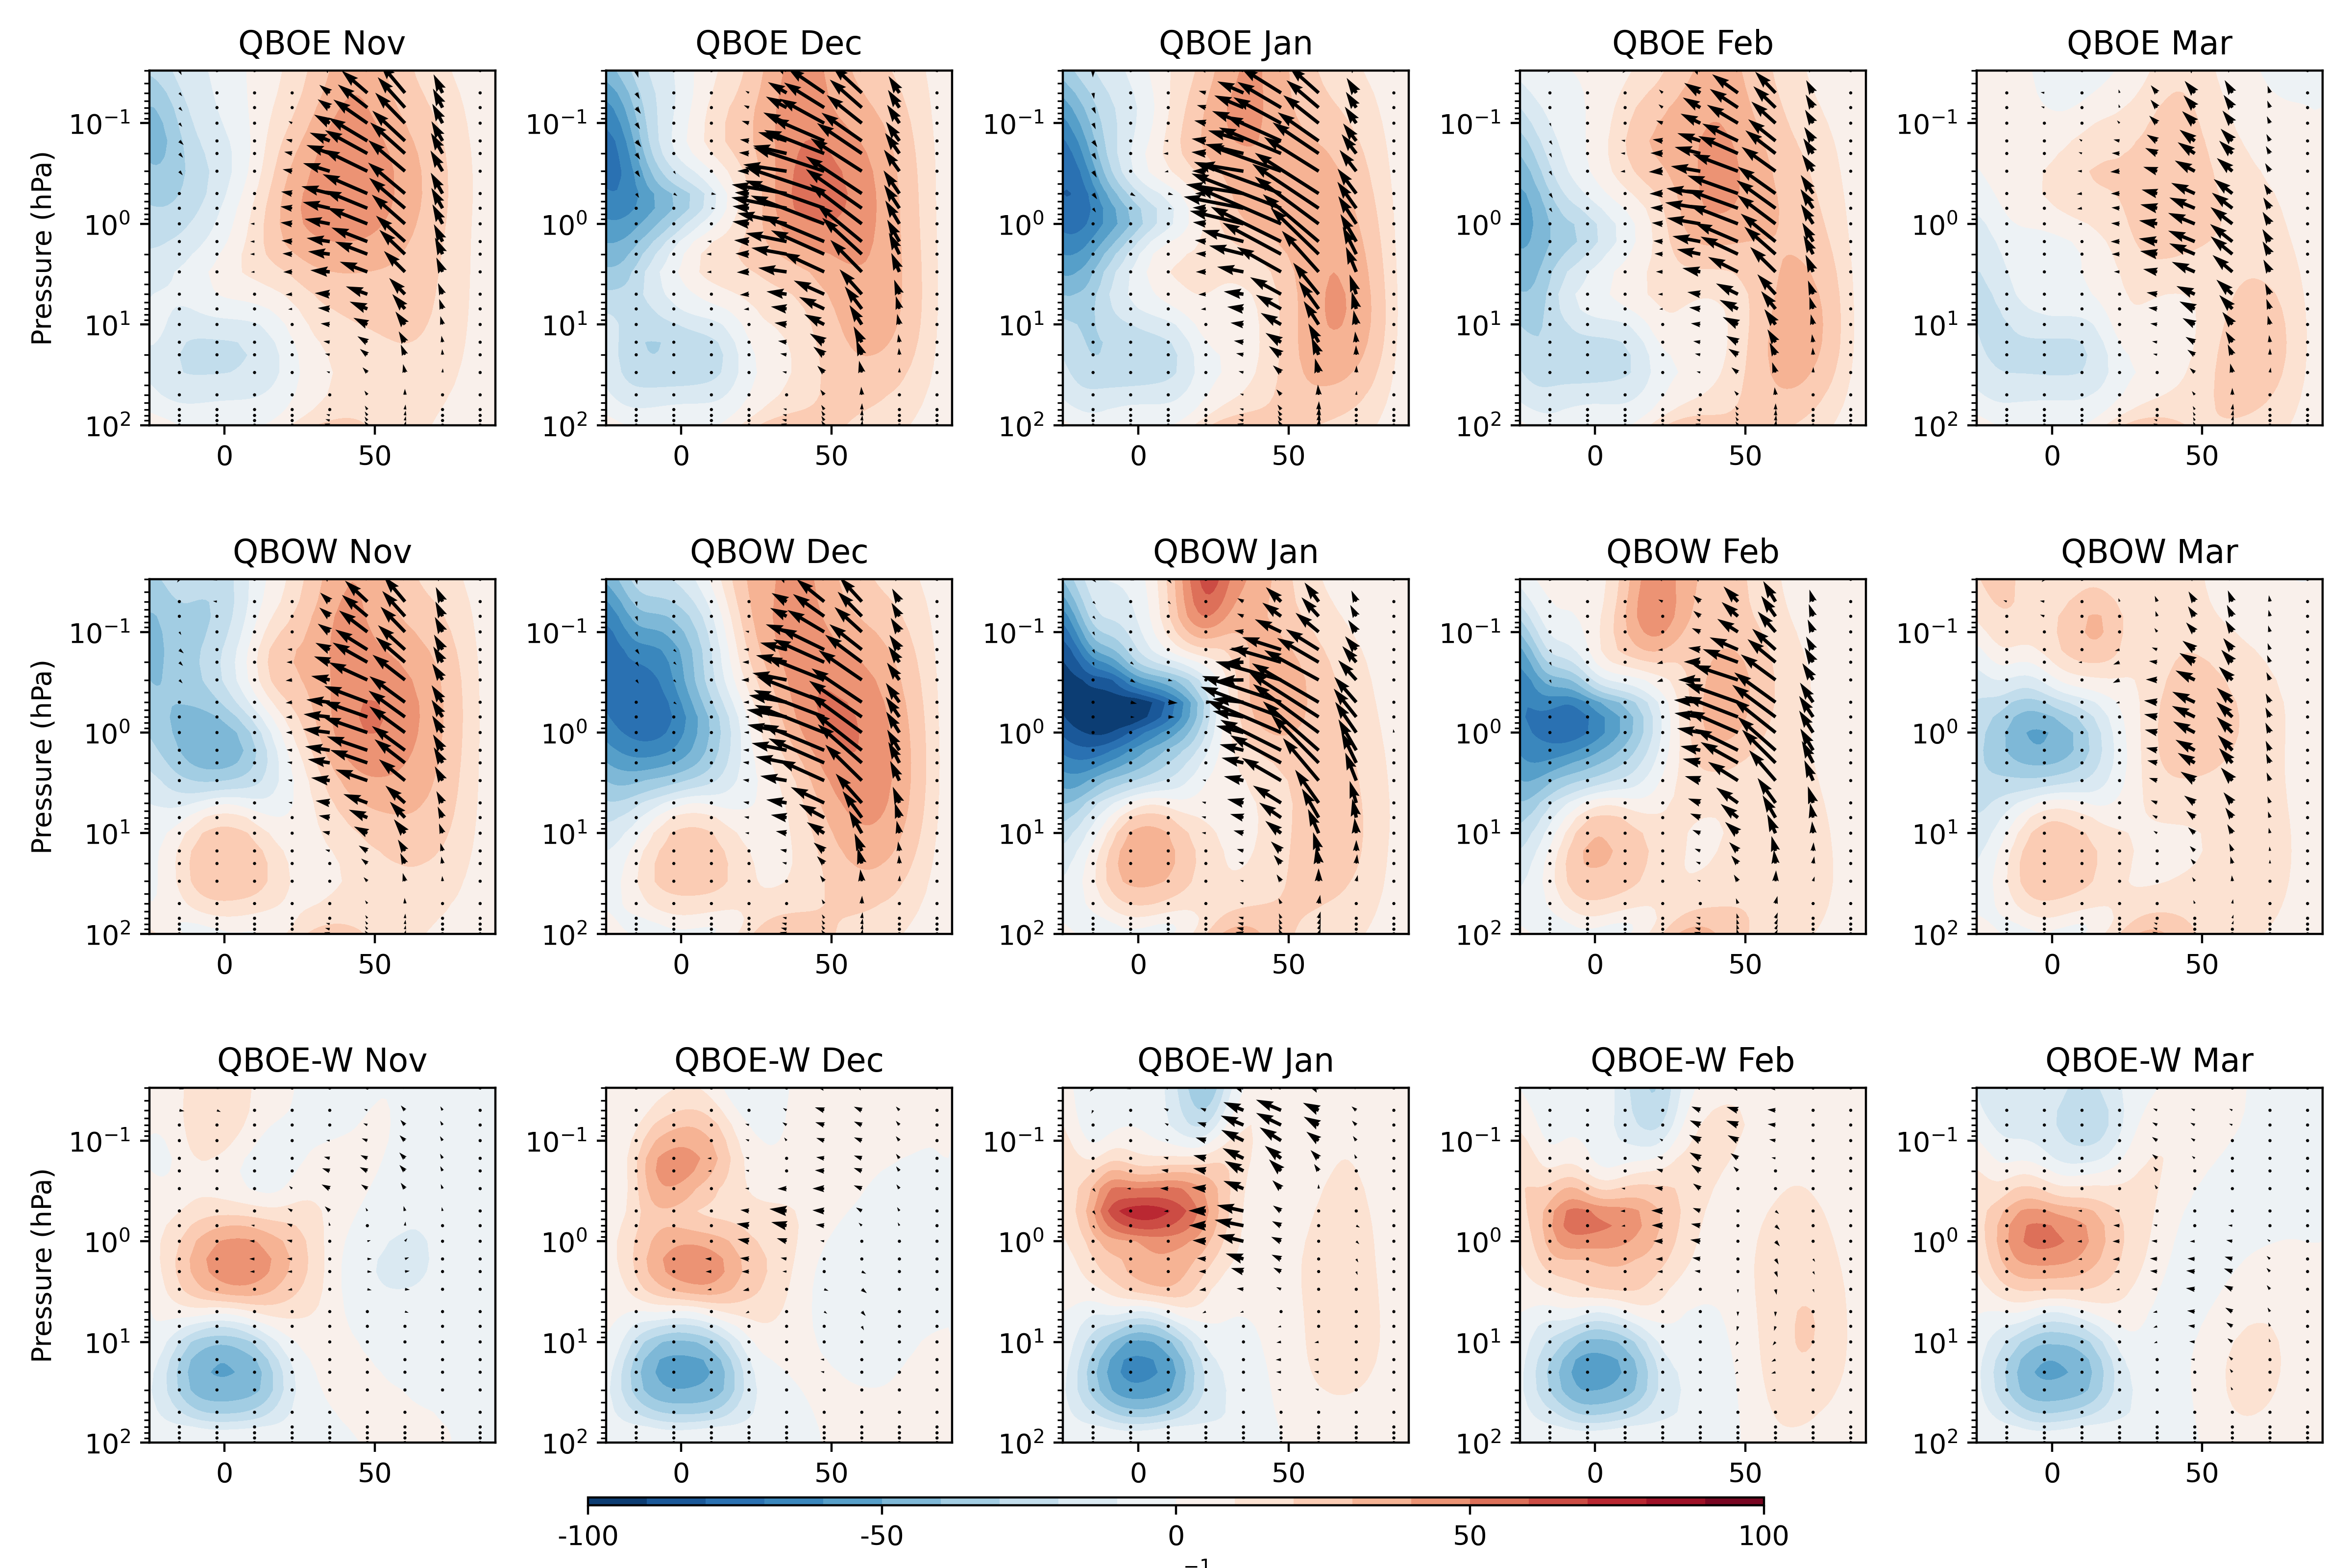
\includegraphics[width = \linewidth]{Figures/Figures-deepQBO/EP_flux_composites_by_month_QBO_phases_d_higher_MarQBO_vs_Mar_30hPa_5thresh.png}
\caption[]{Deep QBO experiment composites of ZMZW (coloured shading) and EP fluxes (arrows with units of $m^2s^{-2}$), which indicate the direction of wave propagation, under QBOE (top row) and QBOW (middle row) conditions as well as the difference between QBOE and QBOW composites (bottom row).}
\label{fig:EP_deep}
\end{center}
\end{figure}
\newpage

\section{Results in the context of previous work}
Our analysis so far indicates that a perpetually deep QBO may enhance the magnitude of teleconnections. It also suggests the importance of a mechanism involving the SAO in accounting for MSLP responses to the QBO in the deep experiment. However, our results are still somewhat surprising and warrant further examination. Namely, it is unclear why the study of \cite{andrewsObserved2019d} obtains an enhanced MSLP response consistent with a HT link using a deep QBO metric which preferentially picks out winters which exhibits a deep QBO while our perpetual deep QBO experiment is dominated by an opposite response in the vortex and MSLP. In this section, we compare the potential mechanisms involved in teleconnections associated with utilising a deep QBO measure in an existing simulation (as \cite{andrewsObserved2019d} does) with our approach which prescribes the QBO depth in tailor made simulations. 

An analogous measure of the effect of a deep QBO metric to that in \cite{andrewsObserved2019d} would be to analyse the UKESM pi-control simulation utilised in chapters 3 and 4. Indeed, \cite{andrewsObserved2019d} use the HadGEM3-GC2 model \citep{williamsMet2018b}, a predecessor of UKESM1, and the length of the simulation (1000 years) allows for robust composite analysis. Figure \ref{fig:SLP_picontrol_50} shows MSLP composites for different QBO conditions using a QBO metric at 50hPa (the standard level as discussed above) from the pi-control simulation. These composites show that this model does not exhibit coherent MSLP anomaly patterns over the Atlantic - there is little to no response in this region to either phase and marginal composite differences (up to $\sim$xxxhPa). A Pacific response is slightly more evident but still only peaks in magnitude at $\sim$1hPa composite difference. There is also an asymmetry in the abundance of QBOE and QBOW months that make up the composites - Significantly more QBOE phases are observed in NH winter which is consistent with similar composite analysis in chapter 3 (figure \ref{fig:SSW_hist_QBO_phase}) in which this feature is discussed further. We compare this single level definition to an analogous plot using the same deep QBO metric as employed by \cite{andrewsObserved2019d}, the average winds between 15hPa and 30hPa. Figure \ref{fig:SLP_picontrol_deep} shows MSLP composites associated with phases of this deep metric and the anomalies associated with each phase are significantly enhanced compared to figure \ref{fig:SLP_picontrol_50}: Clear negative anomalies are visible over the northern mode of the NAO (in the Icelandic region) for QBOW conditions peaking in January and similar anomalies are apparent in February too. There is also a coherent response to the deep QBO in the north Pacific which are first evident in December and increases in magnitude until a peak in February (similar to patterns in this region in the deep experiment). 


\begin{figure}[h!]
\begin{center}
\noindent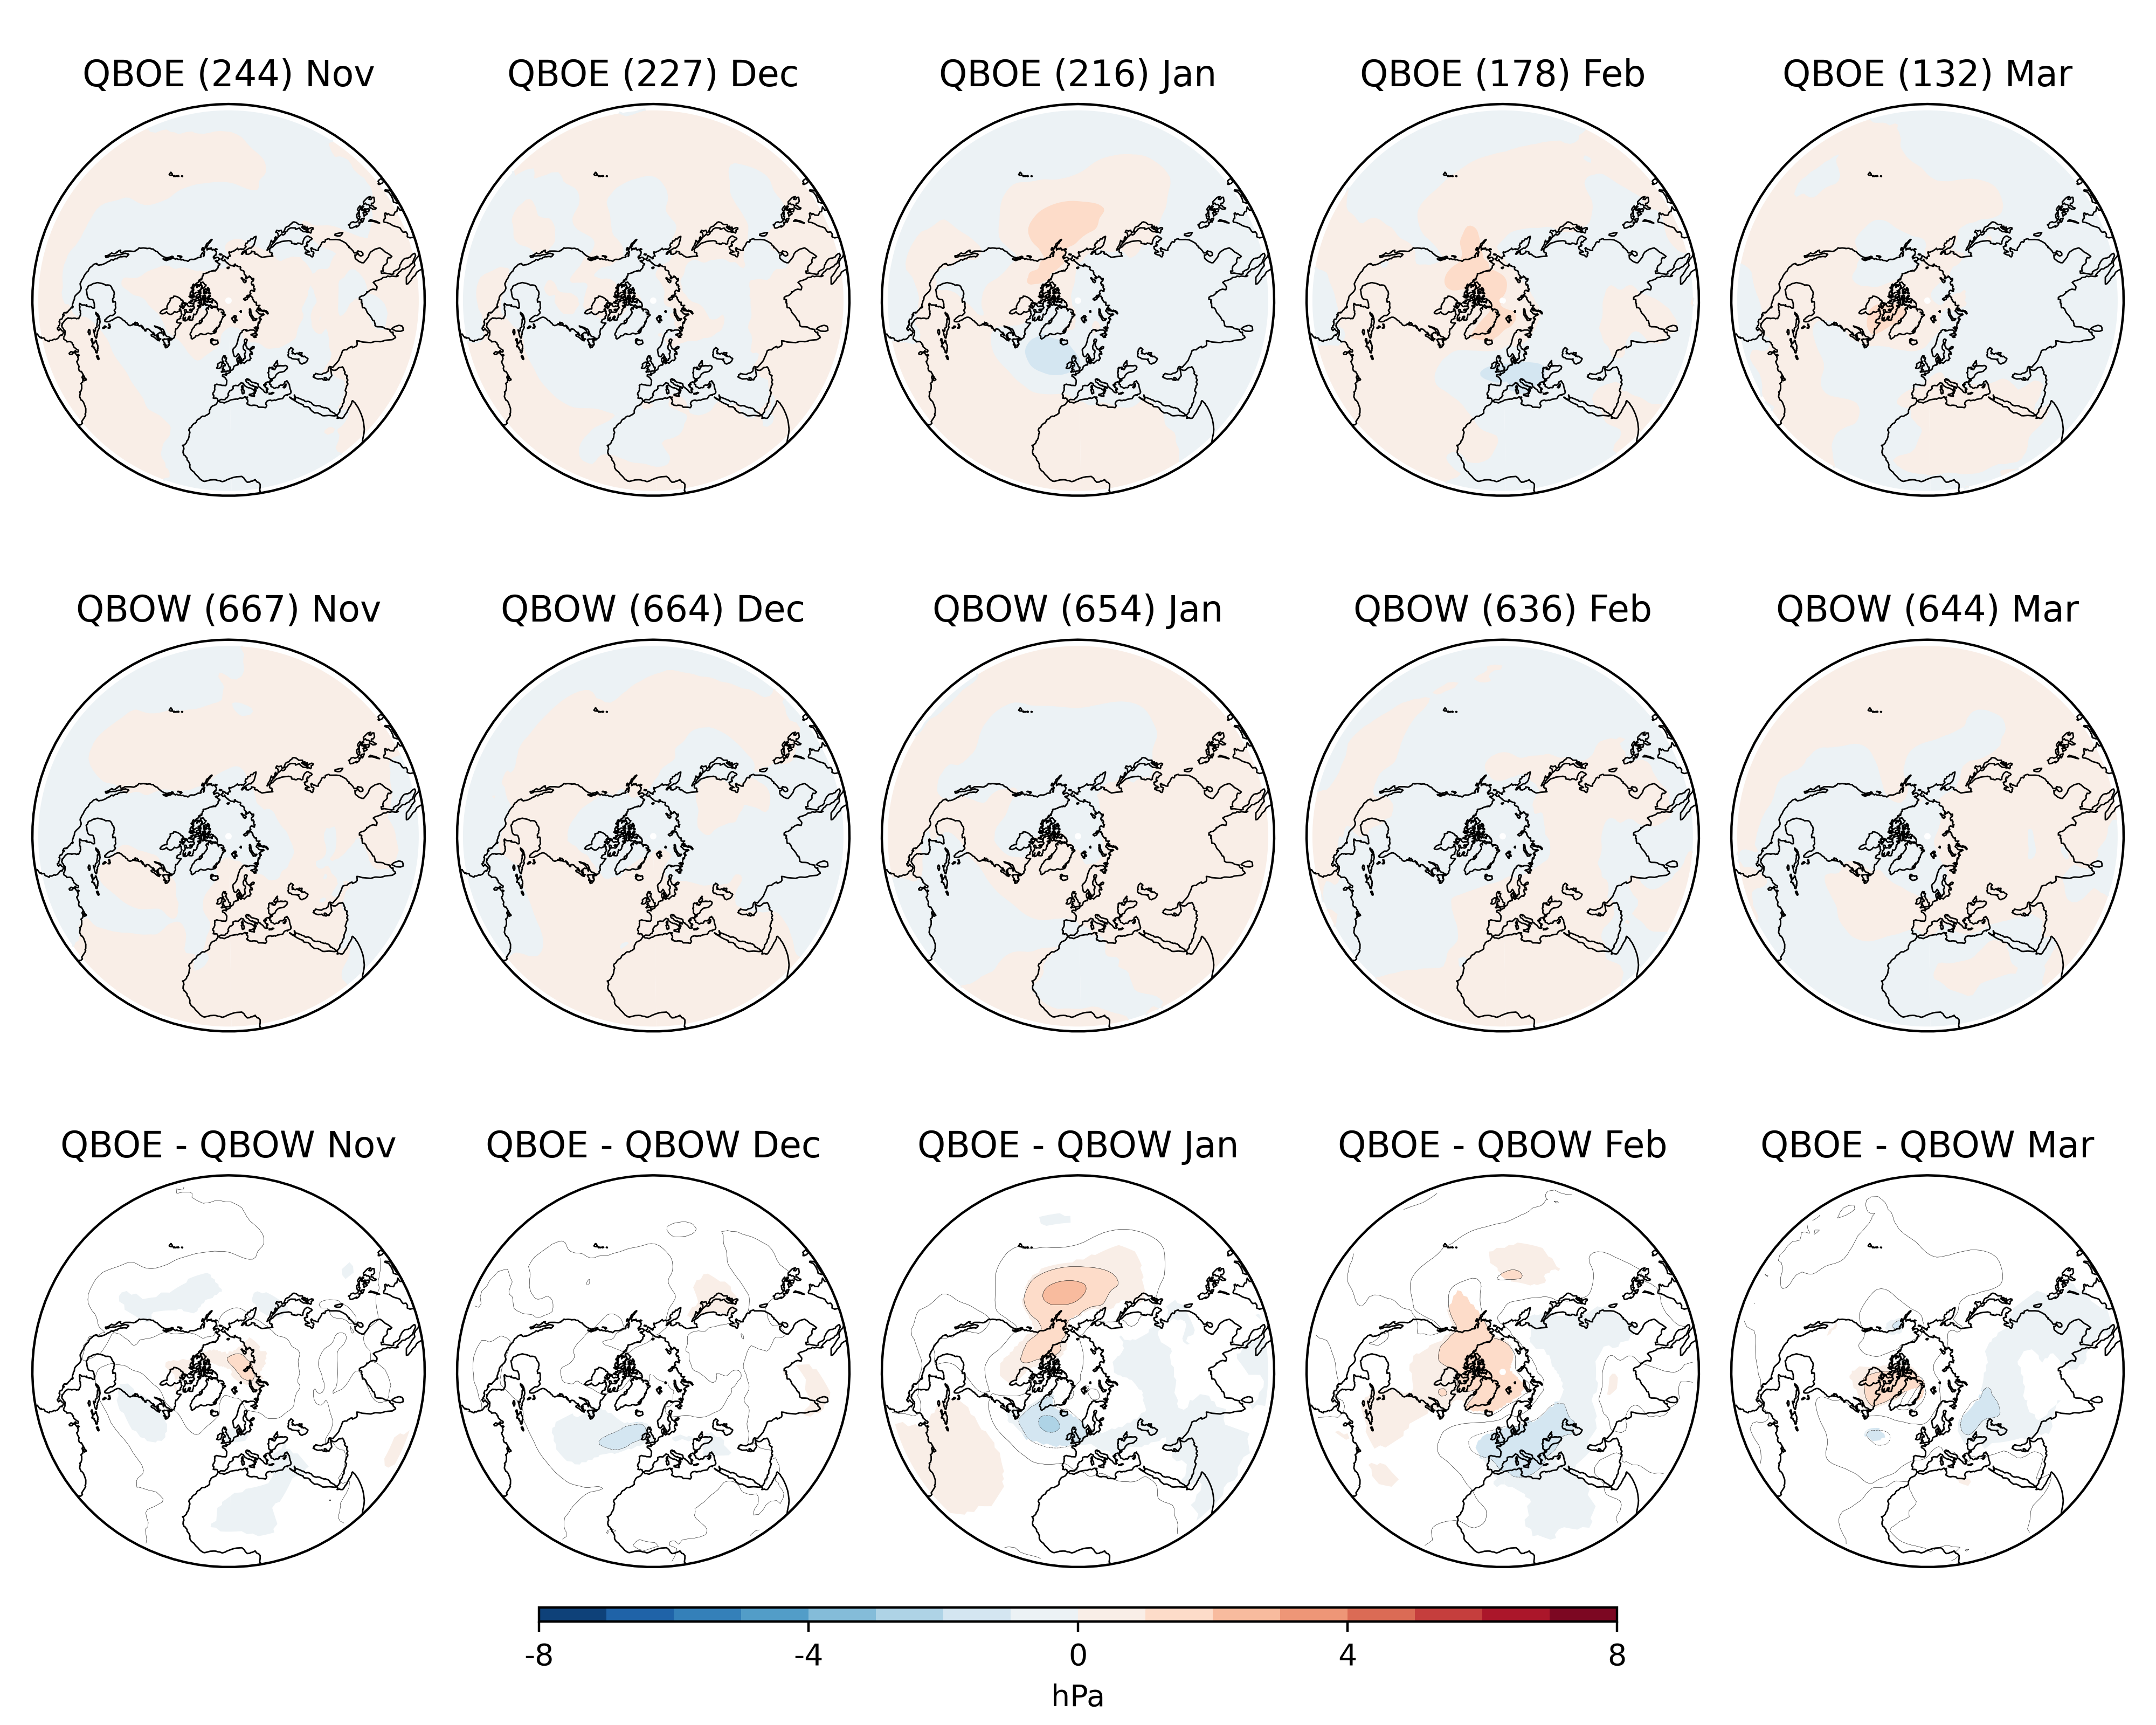
\includegraphics[width = 0.8\linewidth]{Figures/Figures-deepQBO/SLP_composites_individual_months_QBO_phases_U_picontrol_50hPa_5thresh.png}
\caption[]{like figure \ref{fig:SLP_piclim} for the pi-control simulation. QBO phases for each composite are defined as any monthly equatorial ($5^{\circ}$\ S--$5^{\circ}\ $N average) ZMZW that exceeds a magnitude of 5\ m\,s$^{-1}$ on the 50hPa level.}
\label{fig:SLP_picontrol_50}
\end{center}
\end{figure}

\begin{figure}[h!]
\begin{center}
\noindent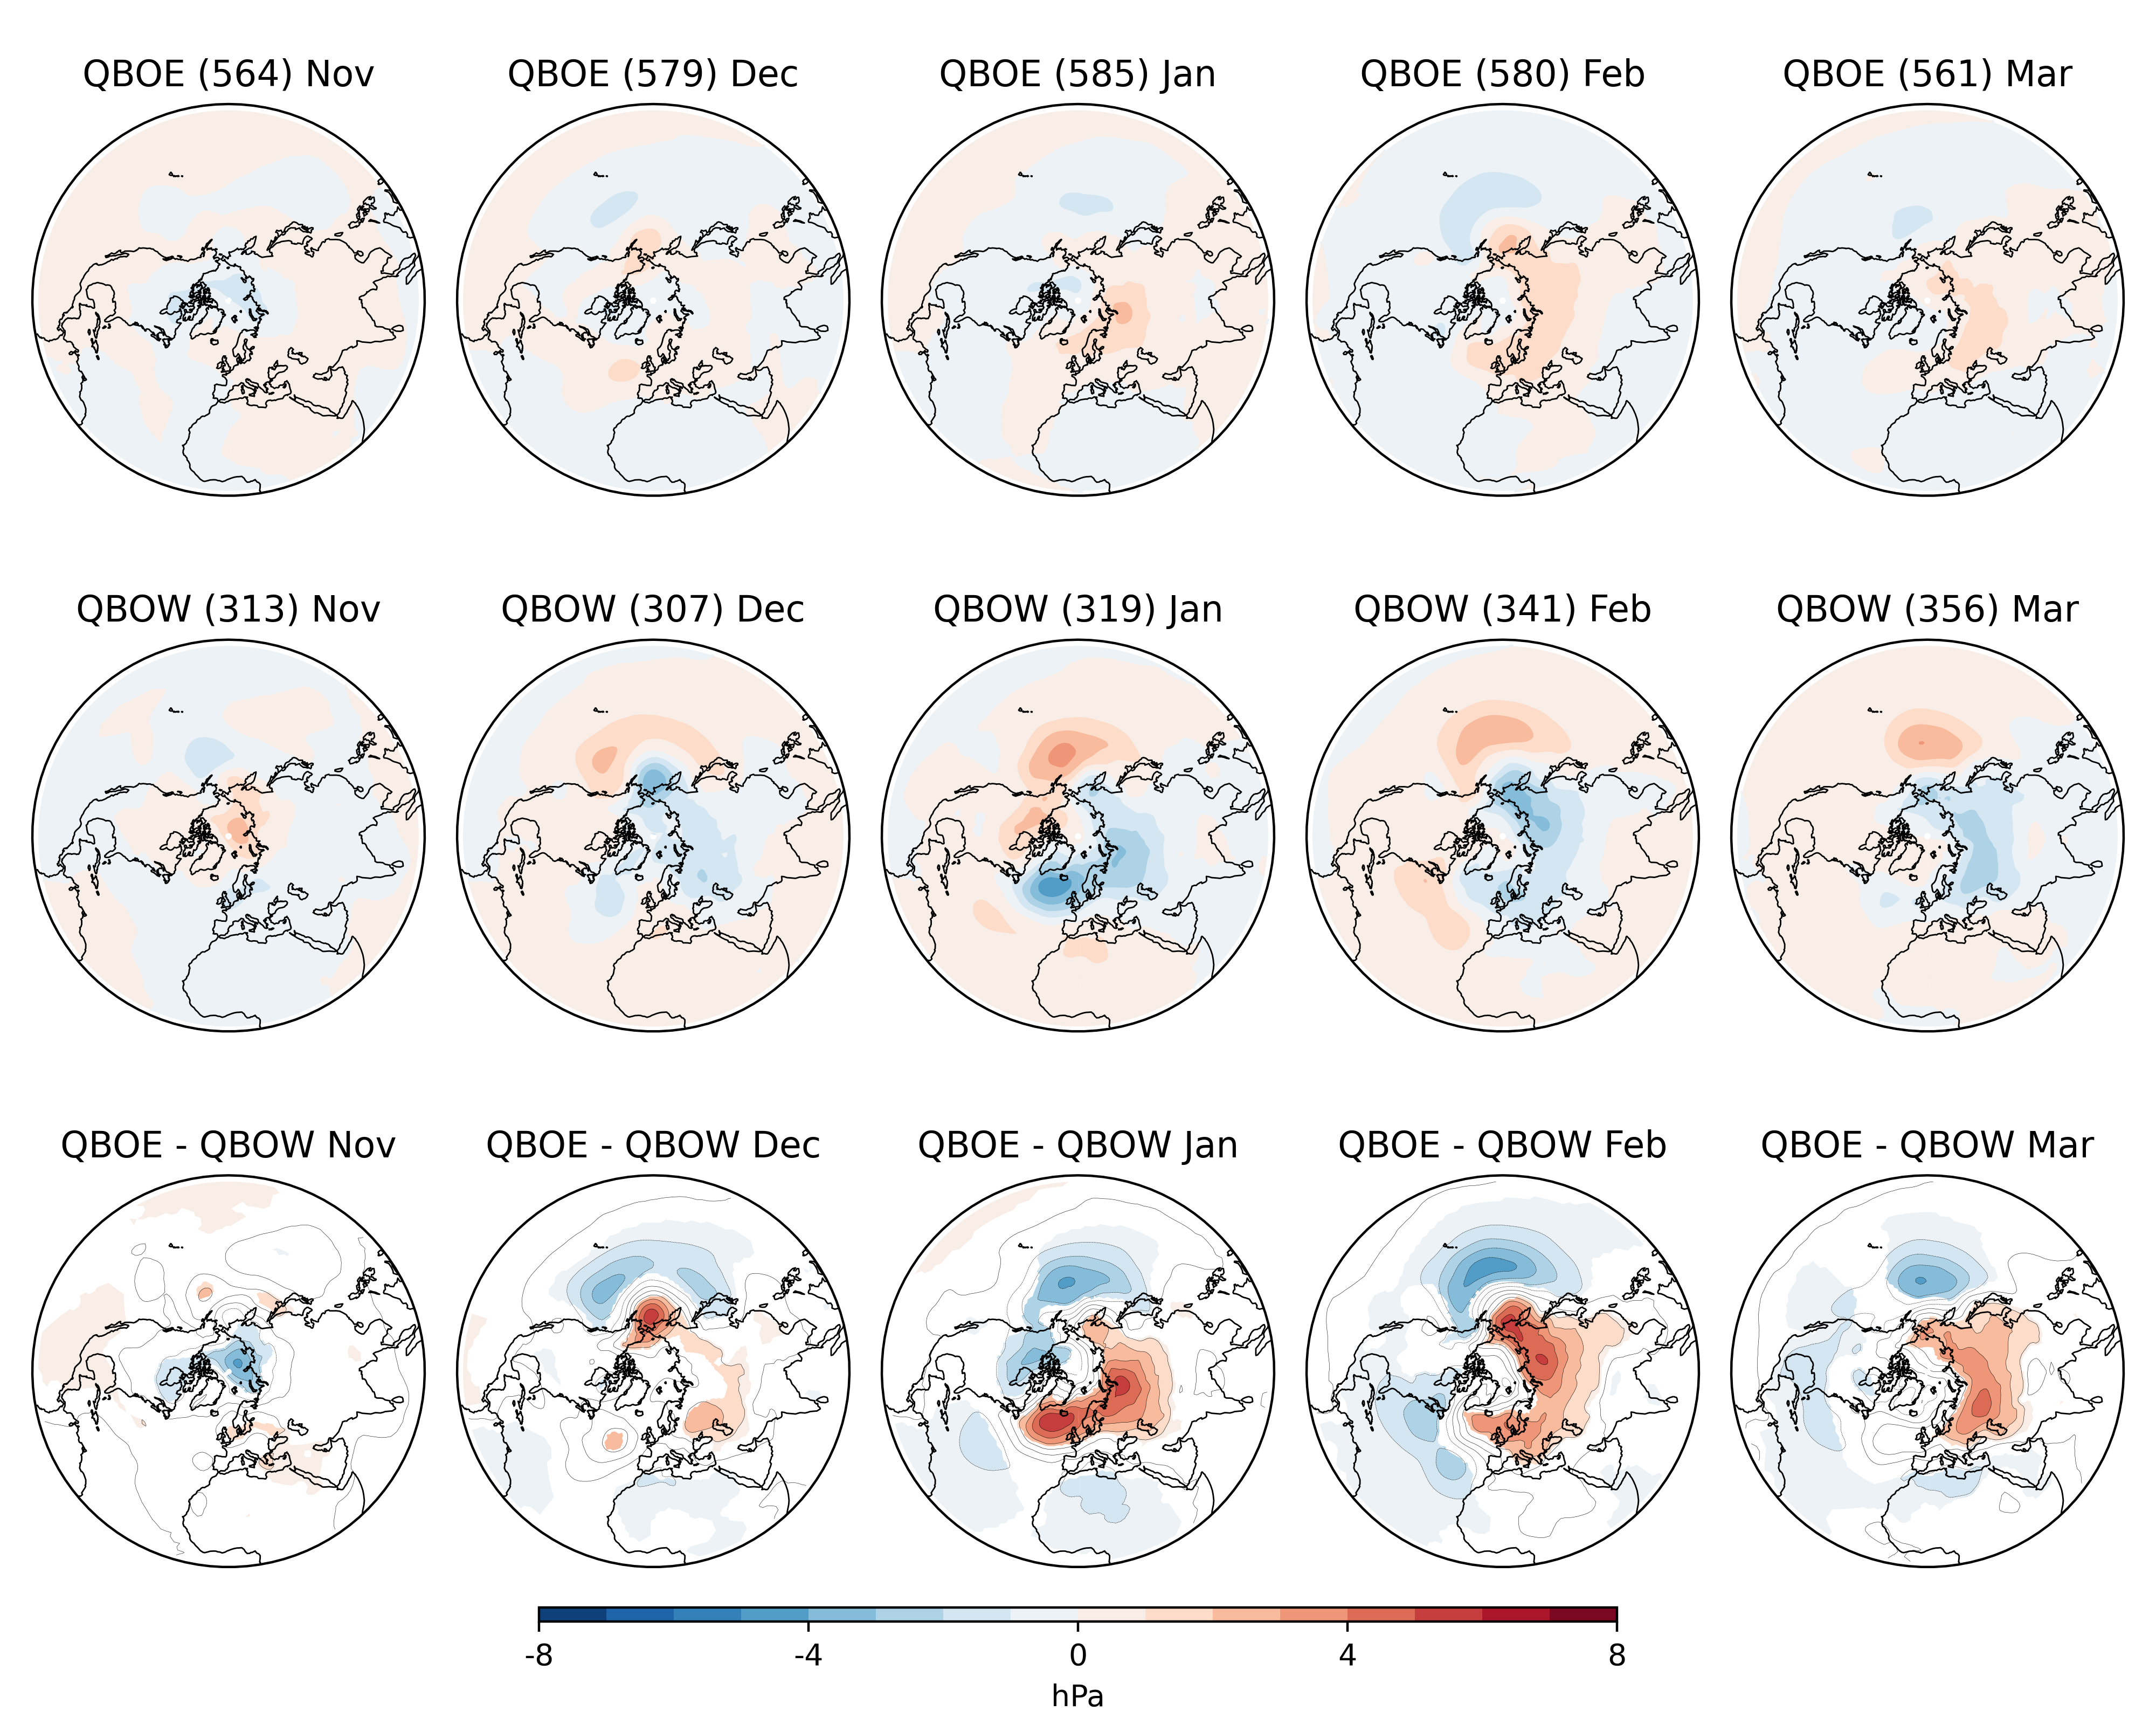
\includegraphics[width = 0.8\linewidth]{Figures/Figures-deepQBO/SLP_composites_individual_months_QBO_phases_U_picontrol_deephPa_5thresh.png}
\caption[]{Like figure \ref{fig:SLP_picontrol_50} but defining QBO phases using the same deep metric as employed in \cite{andrewsObserved2019d}, any monthly equatorial ($5^{\circ}$\ S--$5^{\circ}\ $N average) ZMZW averaged between the 15hPa and 30hPa levels that exceeds a magnitude of 5\ m\,s$^{-1}$.}
\label{fig:SLP_picontrol_deep}
\end{center}
\end{figure}

Importantly, the MSLP responses using the deep QBO metric are consistent with with the results of \cite{andrewsObserved2019d} (their figure 6). Namely, in the NAO region the QBOE (QBOW) phase is associated with positive (negative) anomalies over the Icelandic low and therefore a negative (positive) NAO. The sign of Pacific responses is also consistent with their results; QBOE (QBOW) phase associated with decreased (increased) pressure over the AL region. The pi-control also exhibits QBO-vortex coupling consistent with an expected HT effect - analysis from chapter 3 (figure \ref{fig:holton_tan_comp}) showed a negative composite difference in vortex winds for QBOE-QBOW conditions over the whole winter. There are also significant responses in the SAO region to deep QBO phase. However, these anomalies are significantly lower and cover a smaller region than those in the deep QBO experiment (figure \ref{fig:HT_deep})

is smaller than that in the deep QBO experiment and there are no significant correlations between the vortex and the SAO near 0.3hPa which were a prominent feature of the imposed deep

Interestingly, the magnitude of the vortex response using the deep metric is similar to that exhibited for the 50hPa QBO. A marked difference between the composites however, is the presence of a tropospheric sub-tropical anomaly using the deep metric which is also prominent in the composites of our deep nudged experiment (figure \ref{fig:HT_deep}) but absent in the shallow QBO simulation. This suggests that the enhanced MSLP responses using a deep QBO measure in the pi-control may arise primarily via the subtropical pathway (which is absent using the 50hPa QBO) as opposed to via modulation of the vortex which is comparable using both QBO metrics. 

Alternatively, this result may indicate that the vortex anomalies (e.g. SSWs) associated with a 50hPa metric are, on average, less likely to perturb tropospheric and surface conditions than those associated with deep QBO phases. This is evident from figure \ref{HT_picontrol} which shows that negative composite differences in the vortex fail to extend into the troposphere using the 50hPa QBO but easterly anomalies are apparent in the troposphere and surface near 60N in the deep QBO composites. The presence of the deep QBO leading to greater downward propagation of vortex anomalies is also apparent from our nudged QBO experiments. The point correlations of the vortex shown in figure \ref{fig:point_cors} from the deep QBO experiment (top row) show significant correlations extending vertically downwards from the vortex region into the troposphere and surface whereas no significant correlations are present in these regions for the shallow of pi-clim control simulations (middle and bottom rows). The cause of these differences, both in the pi-control and nudged experiments, are unclear not least because variability in the downward influence of the vortex is not well understood (see section \ref{sec:Downward_influence}) 

\section{Summary and Discussion}

In this chapter, we analysed the role of vertical structure of the QBO in teleconnections with the vortex and surface using a set of relaxation experiments which prescribed different degrees of QBO vertical coherence. While many studies have suggested the importance of QBO metrics which incorporate the vertical structure of the QBO (refs), many of these identify statistical associations between QBO metrics and other climate variability. We are aware of no works that explicitly impose QBO structure to test teleconnections and many of the mechanisms involved are still not fully understood. 

We found that an un-nudged configuration of the model (the pi-clim cntrl) was able to simulate some elements of connection between the QBO and the surface however the MSLP response patterns did not closely resemble that of the NAO or AO and were significantly less coherent and persistent than those reported in previous modelling and observational studies (namely \cite{Andrews2020}).

A simulation which prescribed a QBO with perpetual vertical coherence (the deep QBO experiment) exhibited significantly larger anomalies in MSLP than both the un-nudged simulation and one that prescribed a shallow QBO (with different QBO phases near the 100hPa and 10hPa levels respectively). These large anomalies in the deep experiment corresponded to a positive NAO pattern in late NH winter concentrated over the southern node in the Azores region. Surprisingly, QBOE phases were associated with a positive NAO pattern, an opposite response to that found in studies using a deep QBO metric \citep{Andrews2020} as well as that expected from a pathway involving the vortex (the Holton-Tan association, \cite{holtonNumerical1980}).

We aimed to account for this opposite sign in response by examining the vortex response to QBOs in each experiment. As with the MSLP response, the deep QBO experiment shows greater responses from the vortex to QBO phases than in the deep and un-nudged simulations. These responses also evolve within the NH winter with negative response to QBOE in early winter (in line with an expected HT link) and large amplitude positive responses in Jan-Mar. This switch in vortex response may account for the NAO patterns in late winter - I.E. the positive vortex response in later winter leads to a positive NAO via the vortex's influence over the NAO \citep{charlton-perezInfluence2018e}. 

Additionally we noted that the late winter vortex response in this deep experiment, which was largely absent in the other experiments, was associated with significant late winter SAO anomalies, likely induced via preferential filtering of equatorial waves by the deep QBO phase below. An analysis of EP fluxes in these months revealed that anomalies in the easterly phase of the SAO associated with different QBO phases modulate the equatorward propagation of planetary waves in the upper stratosphere away from the vortex under QBOE conditions leading to a vortex strengthening. This gives a potential mechanism by which later winter MSLP response patterns correspond to positive (negative) NAO under QBOE (QBOW). 

Overall, our experiments indicate that anomalies associated with different QBO phases at the surface and in the vortex region are, on average, enhanced by the presence of a perpetually deep QBO compared to a perpetual shallow QBO and a model whose QBO is allowed to evolve freely. 

It also provides further evidence of the role of the SAO in vortex variability as it appears to modulate the deep QBO's teleconnections in late NH winter. Despite these promising results, we note that some teleconnections appear inconsistent with previous work (namely the SLP response of opposite sign to andrews et al. which is likely caused by a switch in HT sign in late winter) 

Limitations
- Some teleconnections are inconsistent with previous work using deep QBO metrics. While we account for these anomalies in our experiments, the question still remains as to why \cite{andrewsObserved2019d} found opposite NAO responses over the whole season. The cause of this discrepancy is difficult to identify as individual month responses 

    our deep experiment may over-represent the seasonal progression of the HT (too much late winter!). 

    I.E. the perpetually deep QBO may lead to unrealistically large SAO anomalies which inflates the late winter signal. Open question still remains as to why the SAO response in studies using a deep QBO are smaller than in the deep exepriment. 
    
    - Further experiments could impose a shallow and deep QBO as well as a climatological/typical SAO. This may prevent the possible QBO signals being eradicated by the induced SAO anomalies as is the case in the deep simulation here. 

- Only a single model which has biases: 
    notably in QBO period (32 months as opposed to 26-28 in reanalysis) 

    as well as the appearance of November SSWs in all experiments which has the potential to alter the evolution of the vortex throughout the remainder of winter as the vortex recovers from a November disruption. However, we accounted for this bias by removing year containing a November SSW and the results are generally unaffected.

- Perpetual deep and/ or shallow QBO conditions are not realistic. Reanalyses exhibit a QBO with deep and shallow attributes. Our experiments are, nonetheless a useful tool in isolating the effect of these structures on teleconnections and by design may not be fully representative of the real climate system. 


